%%%%%%%%%%%%%%%%%%%%%%%%%%%%%%%%%%%%%%%%%
% Dept. of Computer Science and Information Systems
% Birkbeck, University of London
% Template for MSc dissertations
%  
% Adapted by Y. Prifti, ylli@dcs.bbk.ac.uk;
% A. Provetti ale@dcs.bbk.ac.uk  
% from v. 2.5  
%
% This template was downloaded from:
% http://www.LaTeXTemplates.com
%
% Version 2.x major modifications by:
% Vel (vel@latextemplates.com)
%
% This template is based on a template by:
% Steve Gunn (http://users.ecs.soton.ac.uk/srg/softwaretools/document/templates/)
% Sunil Patel (http://www.sunilpatel.co.uk/thesis-template/)
%
% Template license:
% CC BY-NC-SA 3.0 (http://creativecommons.org/licenses/by-nc-sa/3.0/)
%
%%%%%%%%%%%%%%%%%%%%%%%%%%%%%%%%%%%%%%%%%

%----------------------------------------------------------------------------------------
%	PACKAGES AND OTHER DOCUMENT CONFIGURATIONS
%----------------------------------------------------------------------------------------

\documentclass[
11pt, % The default document font size, options: 10pt, 11pt, 12pt
%oneside, % Two side (alternating margins) for binding by default, uncomment to switch to one side
english, % ngerman for German
singlespacing, % Single line spacing, alternatives: onehalfspacing or doublespacing
%draft, % Uncomment to enable draft mode (no pictures, no links, overfull hboxes indicated)
%nolistspacing, % If the document is onehalfspacing or doublespacing, uncomment this to set spacing in lists to single
%liststotoc, % Uncomment to add the list of figures/tables/etc to the table of contents
%toctotoc, % Uncomment to add the main table of contents to the table of contents
%parskip, % Uncomment to add space between paragraphs
%nohyperref, % Uncomment to not load the hyperref package
headsepline, % Uncomment to get a line under the header
%chapterinoneline, % Uncomment to place the chapter title next to the number on one line
%consistentlayout, % Uncomment to change the layout of the declaration, abstract and acknowledgements pages to match the default layout
]{MastersDoctoralThesis} % The class file specifying the document structure

\usepackage[utf8]{inputenc} % Required for inputting international characters
\usepackage[T1]{fontenc} % Output font encoding for international characters

\usepackage{mathpazo} % Use the Palatino font by default

\usepackage[backend=bibtex,style=authoryear,natbib=true]{biblatex} % Use the bibtex backend with the authoryear citation style (which resembles APA)

\addbibresource{example.bib} % The filename of the bibliography

\usepackage[autostyle=true]{csquotes} % Required to generate language-dependent quotes in the bibliography

\usepackage{color}
\definecolor{editorGray}{rgb}{0.95, 0.95, 0.95}
\definecolor{editorOcher}{rgb}{1, 0.5, 0} % #FF7F00 -> rgb(239, 169, 0)
\definecolor{editorGreen}{rgb}{0, 0.5, 0} % #007C00 -> rgb(0, 124, 0)
\usepackage{upquote}
\usepackage{listings}
\lstdefinelanguage{JavaScript}{
	morekeywords={break, case, catch, continue, debugger, default, delete,         do, else, false, finally, for, function, if, in, instanceof, new, null, return, switch, this, throw, true, try, typeof, var, void, while, with},
	morecomment=[s]{/*}{*/},
	morecomment=[l]//,
	morestring=[b]",
	morestring=[b]'
}
\lstdefinelanguage{CSS}{
	keywords={accelerator,azimuth,background,background-attachment,
		background-color,background-image,background-position,
		background-position-x,background-position-y,background-repeat,
		behavior,border,border-bottom,border-bottom-color,
		border-bottom-style,border-bottom-width,border-collapse,
		border-color,border-left,border-left-color,border-left-style,
		border-left-width,border-right,border-right-color,
		border-right-style,border-right-width,border-spacing,
		border-style,border-top,border-top-color,border-top-style,
		border-top-width,border-width,bottom,caption-side,clear,
		clip,color,content,counter-increment,counter-reset,cue,
		cue-after,cue-before,cursor,direction,display,elevation,
		empty-cells,filter,float,font,font-family,font-size,
		font-size-adjust,font-stretch,font-style,font-variant,
		font-weight,height,ime-mode,include-source,
		layer-background-color,layer-background-image,layout-flow,
		layout-grid,layout-grid-char,layout-grid-char-spacing,
		layout-grid-line,layout-grid-mode,layout-grid-type,left,
		letter-spacing,line-break,line-height,list-style,
		list-style-image,list-style-position,list-style-type,margin,
		margin-bottom,margin-left,margin-right,margin-top,
		marker-offset,marks,max-height,max-width,min-height,
		min-width,-moz-binding,-moz-border-radius,
		-moz-border-radius-topleft,-moz-border-radius-topright,
		-moz-border-radius-bottomright,-moz-border-radius-bottomleft,
		-moz-border-top-colors,-moz-border-right-colors,
		-moz-border-bottom-colors,-moz-border-left-colors,-moz-opacity,
		-moz-outline,-moz-outline-color,-moz-outline-style,
		-moz-outline-width,-moz-user-focus,-moz-user-input,
		-moz-user-modify,-moz-user-select,orphans,outline,
		outline-color,outline-style,outline-width,overflow,
		overflow-X,overflow-Y,padding,padding-bottom,padding-left,
		padding-right,padding-top,page,page-break-after,
		page-break-before,page-break-inside,pause,pause-after,
		pause-before,pitch,pitch-range,play-during,position,quotes,
		-replace,richness,right,ruby-align,ruby-overhang,
		ruby-position,-set-link-source,size,speak,speak-header,
		speak-numeral,speak-punctuation,speech-rate,stress,
		scrollbar-arrow-color,scrollbar-base-color,
		scrollbar-dark-shadow-color,scrollbar-face-color,
		scrollbar-highlight-color,scrollbar-shadow-color,
		scrollbar-3d-light-color,scrollbar-track-color,table-layout,
		text-align,text-align-last,text-decoration,text-indent,
		text-justify,text-overflow,text-shadow,text-transform,
		text-autospace,text-kashida-space,text-underline-position,top,
		unicode-bidi,-use-link-source,vertical-align,visibility,
		voice-family,volume,white-space,widows,width,word-break,
		word-spacing,word-wrap,writing-mode,z-index,zoom},  
	sensitive=true,
	morecomment=[l]{//},
	morecomment=[s]{/*}{*/},
	morestring=[b]',
	morestring=[b]",
	alsoletter={:},
	alsodigit={-}
}
\lstdefinelanguage{HTML5}{
	language=html,
	sensitive=true, 
	alsoletter={<>=-},
	otherkeywords={
		% HTML tags
		<, </, >,
		</a, <a, </a>,
		</abbr, <abbr, </abbr>,
		</address, <address, </address>,
		</area, <area, </area>,
		</area, <area, </area>,
		</article, <article, </article>,
		</aside, <aside, </aside>,
		</audio, <audio, </audio>,
		</audio, <audio, </audio>,
		</b, <b, </b>,
		</base, <base, </base>,
		</bdi, <bdi, </bdi>,
		</bdo, <bdo, </bdo>,
		</blockquote, <blockquote, </blockquote>,
		</body, <body, </body>,
		</br, <br, </br>,
		</button, <button, </button>,
		</canvas, <canvas, </canvas>,
		</caption, <caption, </caption>,
		</cite, <cite, </cite>,
		</code, <code, </code>,
		</col, <col, </col>,
		</colgroup, <colgroup, </colgroup>,
		</data, <data, </data>,
		</datalist, <datalist, </datalist>,
		</dd, <dd, </dd>,
		</del, <del, </del>,
		</details, <details, </details>,
		</dfn, <dfn, </dfn>,
		</div, <div, </div>,
		</dl, <dl, </dl>,
		</dt, <dt, </dt>,
		</em, <em, </em>,
		</embed, <embed, </embed>,
		</fieldset, <fieldset, </fieldset>,
		</figcaption, <figcaption, </figcaption>,
		</figure, <figure, </figure>,
		</footer, <footer, </footer>,
		</form, <form, </form>,
		</h1, <h1, </h1>,
		</h2, <h2, </h2>,
		</h3, <h3, </h3>,
		</h4, <h4, </h4>,
		</h5, <h5, </h5>,
		</h6, <h6, </h6>,
		</head, <head, </head>,
		</header, <header, </header>,
		</hr, <hr, </hr>,
		</html, <html, </html>,
		</i, <i, </i>,
		</iframe, <iframe, </iframe>,
		</img, <img, </img>,
		</input, <input, </input>,
		</ins, <ins, </ins>,
		</kbd, <kbd, </kbd>,
		</keygen, <keygen, </keygen>,
		</label, <label, </label>,
		</legend, <legend, </legend>,
		</li, <li, </li>,
		</link, <link, </link>,
		</main, <main, </main>,
		</map, <map, </map>,
		</mark, <mark, </mark>,
		</math, <math, </math>,
		</menu, <menu, </menu>,
		</menuitem, <menuitem, </menuitem>,
		</meta, <meta, </meta>,
		</meter, <meter, </meter>,
		</nav, <nav, </nav>,
		</noscript, <noscript, </noscript>,
		</object, <object, </object>,
		</ol, <ol, </ol>,
		</optgroup, <optgroup, </optgroup>,
		</option, <option, </option>,
		</output, <output, </output>,
		</p, <p, </p>,
		</param, <param, </param>,
		</pre, <pre, </pre>,
		</progress, <progress, </progress>,
		</q, <q, </q>,
		</rp, <rp, </rp>,
		</rt, <rt, </rt>,
		</ruby, <ruby, </ruby>,
		</s, <s, </s>,
		</samp, <samp, </samp>,
		</script, <script, </script>,
		</section, <section, </section>,
		</select, <select, </select>,
		</small, <small, </small>,
		</source, <source, </source>,
		</span, <span, </span>,
		</strong, <strong, </strong>,
		</style, <style, </style>,
		</summary, <summary, </summary>,
		</sup, <sup, </sup>,
		</svg, <svg, </svg>,
		</table, <table, </table>,
		</tbody, <tbody, </tbody>,
		</td, <td, </td>,
		</template, <template, </template>,
		</textarea, <textarea, </textarea>,
		</tfoot, <tfoot, </tfoot>,
		</th, <th, </th>,
		</thead, <thead, </thead>,
		</time, <time, </time>,
		</title, <title, </title>,
		</tr, <tr, </tr>,
		</track, <track, </track>,
		</u, <u, </u>,
		</ul, <ul, </ul>,
		</var, <var, </var>,
		</video, <video, </video>,
		</wbr, <wbr, </wbr>,
		/>, <!
	},  
	ndkeywords={
		% General
		=,
		% HTML attributes
		accept=, accept-charset=, accesskey=, action=, align=, alt=, async=, autocomplete=, autofocus=, autoplay=, autosave=, bgcolor=, border=, buffered=, challenge=, charset=, checked=, cite=, class=, code=, codebase=, color=, cols=, colspan=, content=, contenteditable=, contextmenu=, controls=, coords=, data=, datetime=, default=, defer=, dir=, dirname=, disabled=, download=, draggable=, dropzone=, enctype=, for=, form=, formaction=, headers=, height=, hidden=, high=, href=, hreflang=, http-equiv=, icon=, id=, ismap=, itemprop=, keytype=, kind=, label=, lang=, language=, list=, loop=, low=, manifest=, max=, maxlength=, media=, method=, min=, multiple=, name=, novalidate=, open=, optimum=, pattern=, ping=, placeholder=, poster=, preload=, pubdate=, radiogroup=, readonly=, rel=, required=, reversed=, rows=, rowspan=, sandbox=, scope=, scoped=, seamless=, selected=, shape=, size=, sizes=, span=, spellcheck=, src=, srcdoc=, srclang=, start=, step=, style=, summary=, tabindex=, target=, title=, type=, usemap=, value=, width=, wrap=,
		% CSS properties
		accelerator:,azimuth:,background:,background-attachment:,
		background-color:,background-image:,background-position:,
		background-position-x:,background-position-y:,background-repeat:,
		behavior:,border:,border-bottom:,border-bottom-color:,
		border-bottom-style:,border-bottom-width:,border-collapse:,
		border-color:,border-left:,border-left-color:,border-left-style:,
		border-left-width:,border-right:,border-right-color:,
		border-right-style:,border-right-width:,border-spacing:,
		border-style:,border-top:,border-top-color:,border-top-style:,
		border-top-width:,border-width:,bottom:,caption-side:,clear:,
		clip:,color:,content:,counter-increment:,counter-reset:,cue:,
		cue-after:,cue-before:,cursor:,direction:,display:,elevation:,
		empty-cells:,filter:,float:,font:,font-family:,font-size:,
		font-size-adjust:,font-stretch:,font-style:,font-variant:,
		font-weight:,height:,ime-mode:,include-source:,
		layer-background-color:,layer-background-image:,layout-flow:,
		layout-grid:,layout-grid-char:,layout-grid-char-spacing:,
		layout-grid-line:,layout-grid-mode:,layout-grid-type:,left:,
		letter-spacing:,line-break:,line-height:,list-style:,
		list-style-image:,list-style-position:,list-style-type:,margin:,
		margin-bottom:,margin-left:,margin-right:,margin-top:,
		marker-offset:,marks:,max-height:,max-width:,min-height:,
		min-width:,transition-duration:,transition-property:,
		transition-timing-function:,transform:,
		-moz-transform:,-moz-binding:,-moz-border-radius:,
		-moz-border-radius-topleft:,-moz-border-radius-topright:,
		-moz-border-radius-bottomright:,-moz-border-radius-bottomleft:,
		-moz-border-top-colors:,-moz-border-right-colors:,
		-moz-border-bottom-colors:,-moz-border-left-colors:,-moz-opacity:,
		-moz-outline:,-moz-outline-color:,-moz-outline-style:,
		-moz-outline-width:,-moz-user-focus:,-moz-user-input:,
		-moz-user-modify:,-moz-user-select:,orphans:,outline:,
		outline-color:,outline-style:,outline-width:,overflow:,
		overflow-X:,overflow-Y:,padding:,padding-bottom:,padding-left:,
		padding-right:,padding-top:,page:,page-break-after:,
		page-break-before:,page-break-inside:,pause:,pause-after:,
		pause-before:,pitch:,pitch-range:,play-during:,position:,quotes:,
		-replace:,richness:,right:,ruby-align:,ruby-overhang:,
		ruby-position:,-set-link-source:,size:,speak:,speak-header:,
		speak-numeral:,speak-punctuation:,speech-rate:,stress:,
		scrollbar-arrow-color:,scrollbar-base-color:,
		scrollbar-dark-shadow-color:,scrollbar-face-color:,
		scrollbar-highlight-color:,scrollbar-shadow-color:,
		scrollbar-3d-light-color:,scrollbar-track-color:,table-layout:,
		text-align:,text-align-last:,text-decoration:,text-indent:,
		text-justify:,text-overflow:,text-shadow:,text-transform:,
		text-autospace:,text-kashida-space:,text-underline-position:,top:,
		unicode-bidi:,-use-link-source:,vertical-align:,visibility:,
		voice-family:,volume:,white-space:,widows:,width:,word-break:,
		word-spacing:,word-wrap:,writing-mode:,z-index:,zoom:
	},  
	morecomment=[s]{<!--}{-->},
	tag=[s]
}

\lstset{%
	% Basic design
	backgroundcolor=\color{editorGray},
	basicstyle={\small\ttfamily},   
	frame=l,
	% Line numbers
	xleftmargin={0.75cm},
	numbers=left,
	stepnumber=1,
	firstnumber=1,
	numberfirstline=true,
	% Code design   
	keywordstyle=\color{blue}\bfseries,
	commentstyle=\color{darkgray}\ttfamily,
	ndkeywordstyle=\color{editorGreen}\bfseries,
	stringstyle=\color{editorOcher},
	% Code
	language=HTML5,
	alsodigit={.:;},
	tabsize=2,
	showtabs=false,
	showspaces=false,
	showstringspaces=false,
	extendedchars=true,
	breaklines=true,        
}

\lstdefinestyle{sharpc}{language=[Sharp]C, frame=lr, rulecolor=\color{blue!80!black}}




%----------------------------------------------------------------------------------------
%	MARGIN SETTINGS
%----------------------------------------------------------------------------------------

\geometry{
	paper=a4paper, % Change to letterpaper for US letter
	inner=2.5cm, % Inner margin
	outer=3.8cm, % Outer margin
	bindingoffset=.5cm, % Binding offset
	top=1.5cm, % Top margin
	bottom=1.5cm, % Bottom margin
	%showframe, % Uncomment to show how the type block is set on the page
}

%----------------------------------------------------------------------------------------
%	THESIS INFORMATION
%----------------------------------------------------------------------------------------


\thesistitle{ Mapping London House Prices through Well-being} % Your thesis title, this is used in the title and abstract, print it elsewhere with \ttitle

\supervisor{Dr. Alessandro \textsc{Provetti}} % Your supervisor's name, this is used in the title page, print it elsewhere with \supname

\examiner{} % Your examiner's name, this is not currently used anywhere in the template, print it elsewhere with \examname

\degree{Master of Science} % Your degree name, this is used in the title page and abstract, print it elsewhere with \degreename

\author{Ben \textsc{Candy}} % Your name, this is used in the title page and abstract, print it elsewhere with \authorname

\addresses{} % Your address, this is not currently used anywhere in the template, print it elsewhere with \addressname

\subject{Data Science} % Your subject area, this is not currently used anywhere in the template, print it elsewhere with \subjectname

\keywords{} % Keywords for your thesis, this is not currently used anywhere in the template, print it elsewhere with \keywordnames

\university{\href{http://www.bbk.ac.uk}{Birkbeck, University of London}} % Your university's name and URL, this is used in the title page and abstract, print it elsewhere with \univname

\department{\href{http://www.dcs.bbk.ac.uk}{Department of Computer Science and Information Systems}} % Your department's name and URL, this is used in the title page and abstract, print it elsewhere with \deptname

\group{} % Your research group's name and URL, this is used in the title page, print it elsewhere with \groupname


\faculty{\href{http://www.bbk.ac.uk/business/}{School of Business, Economics and Informatics}} % Your faculty's name and URL, this is used in the title page and abstract, print it elsewhere with \facname


\AtBeginDocument{
	\hypersetup{pdftitle=\ttitle} % Set the PDF's title to your title
	\hypersetup{pdfauthor=\authorname} % Set the PDF's author to your name
	\hypersetup{pdfkeywords=\keywordnames} % Set the PDF's keywords to your keywords
}

\begin{document}
	
	\frontmatter % Use Roman page numbering style (i, ii, iii, iv...) for the pre-content pages
	
	\pagestyle{plain} % Default to the plain heading style until the thesis style is called for the body content
	
	%----------------------------------------------------------------------------------------
	%	TITLE PAGE
	%----------------------------------------------------------------------------------------
	
	\begin{titlepage}
		\begin{center}
			
			\vspace*{.06\textheight}
			{\scshape\LARGE \univname\par}\vspace{1.5cm} % University name
			\textsc{\Large Master Project Report}\\[0.5cm] % Thesis type
			
			\HRule \\[0.4cm] % Horizontal line
			{\huge \bfseries \ttitle\par}\vspace{0.4cm} % Thesis title
			\HRule \\[1.5cm] % Horizontal line
			
			\begin{minipage}[t]{0.4\textwidth}
				\begin{flushleft} \large
					\emph{Author:}\\
					\href{https://uk.linkedin.com/in/ylliprifti}{\authorname} % Author name - remove the \href bracket to remove the link
				\end{flushleft}
			\end{minipage}
			\begin{minipage}[t]{0.4\textwidth}
				\begin{flushright} \large
					\emph{Supervisor:} \\
					\href{https://www.dcs.bbk.ac.uk/about-us/people/academic-staff/alessandro/}{\supname} % Supervisor name - remove the \href bracket to remove the link  
				\end{flushright}
			\end{minipage}\\[3cm]
			
			
\includegraphics[scale=1.5]{figures/Birkbeck-Logo-Colour} % University/department logo - uncomment to place it
			
			\vfill
			
			\large \textit{A project report submitted in fulfillment of the requirements\\ for the degree of \degreename}\\[0.3cm] % University requirement text
			\textit{in the}\\[0.4cm]
			\deptname\\[2cm] % Research group name and department name
			
			\vfill
			
			{\large \today}\\[4cm] % Date
			
			
			\vfill
		\end{center}
	\end{titlepage}


%----------------------------------------------------------------------------------------
%	DECLARATION PAGE
%----------------------------------------------------------------------------------------

\begin{declaration}
\addchaptertocentry{\authorshipname} % Add the declaration to the table of contents
\noindent I, \authorname, confirm that:

\begin{itemize} 
\item This report is substantially the result of my own work, expressed in my own words, except where explicitly indicated in the text. 
\item I give my permission for it to be submitted to the JISC Plagiarism Detection Service. 
\item 
\item The report may be freely copied and distributed provided the source is explicitly acknowledged.\\
\end{itemize}
 
\noindent Signed:\\
\rule[0.5em]{25em}{0.5pt} % This prints a line for the signature
 
\noindent Date:\\
\rule[0.5em]{25em}{0.5pt} % This prints a line to write the date
\end{declaration}

\cleardoublepage

%----------------------------------------------------------------------------------------
%	QUOTATION PAGE
%----------------------------------------------------------------------------------------

\vspace*{0.2\textheight}

\noindent\enquote{\itshape }\bigbreak

\hfill 

%----------------------------------------------------------------------------------------
%	ABSTRACT PAGE
%----------------------------------------------------------------------------------------

\begin{abstract}
\addchaptertocentry{\abstractname} % Add the abstract to the table of contents
The Thesis Abstract is written here (and usually kept to just this page). The page is kept centered vertically so can expand into the blank space above the title too\ldots
\end{abstract}

%----------------------------------------------------------------------------------------
%	ACKNOWLEDGEMENTS
%----------------------------------------------------------------------------------------

\begin{acknowledgements}
\addchaptertocentry{\acknowledgementname} % Add the acknowledgements to the table of contents
I would like to thank my project supervisor Professor Alessandro Provetti for his support and guidance throughout this project.\ldots
\end{acknowledgements}

%----------------------------------------------------------------------------------------
%	LIST OF CONTENTS/FIGURES/TABLES PAGES
%----------------------------------------------------------------------------------------

\tableofcontents % Prints the main table of contents

\listoffigures % Prints the list of figures

\listoftables % Prints the list of tables

%----------------------------------------------------------------------------------------
%	ABBREVIATIONS
%----------------------------------------------------------------------------------------

\begin{abbreviations}{ll} % Include a list of abbreviations (a table of two columns)

\textbf{LAH} & \textbf{L}ist \textbf{A}bbreviations \textbf{H}ere\\
\textbf{WSF} & \textbf{W}hat (it) \textbf{S}tands \textbf{F}or\\

\end{abbreviations}

%----------------------------------------------------------------------------------------
%	PHYSICAL CONSTANTS/OTHER DEFINITIONS
%----------------------------------------------------------------------------------------

\begin{constants}{lr@{${}={}$}l} % The list of physical constants is a three column table

% The \SI{}{} command is provided by the siunitx package, see its documentation for instructions on how to use it

Speed of Light & $c_{0}$ & \SI{2.99792458e8}{\meter\per\second} (exact)\\
%Constant Name & $Symbol$ & $Constant Value$ with units\\

\end{constants}

%----------------------------------------------------------------------------------------
%	SYMBOLS
%----------------------------------------------------------------------------------------

\begin{symbols}{lll} % Include a list of Symbols (a three column table)

$a$ & distance & \si{\meter} \\
$P$ & power & \si{\watt} (\si{\joule\per\second}) \\
%Symbol & Name & Unit \\

\addlinespace % Gap to separate the Roman symbols from the Greek

$\omega$ & angular frequency & \si{\radian} \\

\end{symbols}

%----------------------------------------------------------------------------------------
%	DEDICATION
%----------------------------------------------------------------------------------------

\dedicatory{For/Dedicated to/To my\ldots} 

%----------------------------------------------------------------------------------------
%	THESIS CONTENT - CHAPTERS
%----------------------------------------------------------------------------------------

\mainmatter % Begin numeric (1,2,3...) page numbering

\pagestyle{thesis} % Return the page headers back to the "thesis" style

% Include the chapters of the thesis as separate files from the Chapters folder
% Uncomment the lines as you write the chapters

% Chapter Template

\chapter{Introduction} % Main chapter title

\label{Chapter1} % Change X to a consecutive number; for referencing this chapter elsewhere, use \ref{ChapterX}

%----------------------------------------------------------------------------------------
%	SECTION 1
%----------------------------------------------------------------------------------------

\section{Motivations and problem statement}

In recent years, the concept of well-being has been the subject of increasing interests for governments, councils, policy makers and researchers, though research on the subject has been happening since the 1970s.
An interesting recent development is a report into well-being in Danish cities by (\cite {OECD16}) which highlights how well-being tools have become an important tool to identify the needs of citizens and the domains where demand for progress is greatest. 

This idea of well-being is often defined using a set of indicators relating to a particular place. There is no universally agreed definition of exactly which factors are the best measures of well-being, however, various indexes and studies show a great deal of commonality on the types of measures that are important to the well-being of citizens.

What is less clear is whether, and how, these indicators affect the real estate values in a specific city. For example, The Greater London Authority created a set of well-being indicators and used them to create a map of well-being by London Ward in 2014 (\cite{GLA14}), however, this was not linked back to real estate values.
In one study looking at linkages between house prices and mental wellbeing, (\cite {AR13}), points out that when people can move freely, each person will maximize wellbeing by moving to areas that best satisfy their preferences; this results in zero correlation between area characteristics (or house prices) and wellbeing. But if people think they are paying too much for poor quality or too little for high quality, we would observe a positive relationship between area characteristics and wellbeing. The study found a positive correlation between house prices and mental wellbeing.

Another hypothesis found in the Economics literature is that real estate values are the drivers of the well-being indicators, happier people are better at generating wealth (\cite {LKD05}), which leaves open the possibility that areas with high well-being provide a flow of people migrating to places with higher real estate values. From the point of view of Data Science it would be interesting to consider the real estate values in bandings such as quintiles as well-being indicators may have a very different relationship with the top 20 percent of areas by real estate value than with areas in the lower four quintiles.

Work on urban scaling (\cite {BLSW10}) suggests that different types of well-being indicators may have different relationships with real estate values due to the non-linear nature of agglomeration. Bettencourt et al. argues that city indicators are governed by power laws rather than linear per-capita indicators. Social factors tend to be superlinear whereas material infrastructure tends to be sublinear at best. There may therefore be some level of divergence between different well-being factors.
This project focuses on the city of London and tries to determine which well-being indicators show a relationship with real-estate values. The findings will be displayed in the form of an interactive map.

This project sets out to create a set of well-being indicators for each administrative ward in London and will attempt to model median house prices based on these indicators.


%----------------------------------------------------------------------------------------
%	SECTION 2
%----------------------------------------------------------------------------------------

\section{Project trailer}

\begin{figure}[H]
\centering
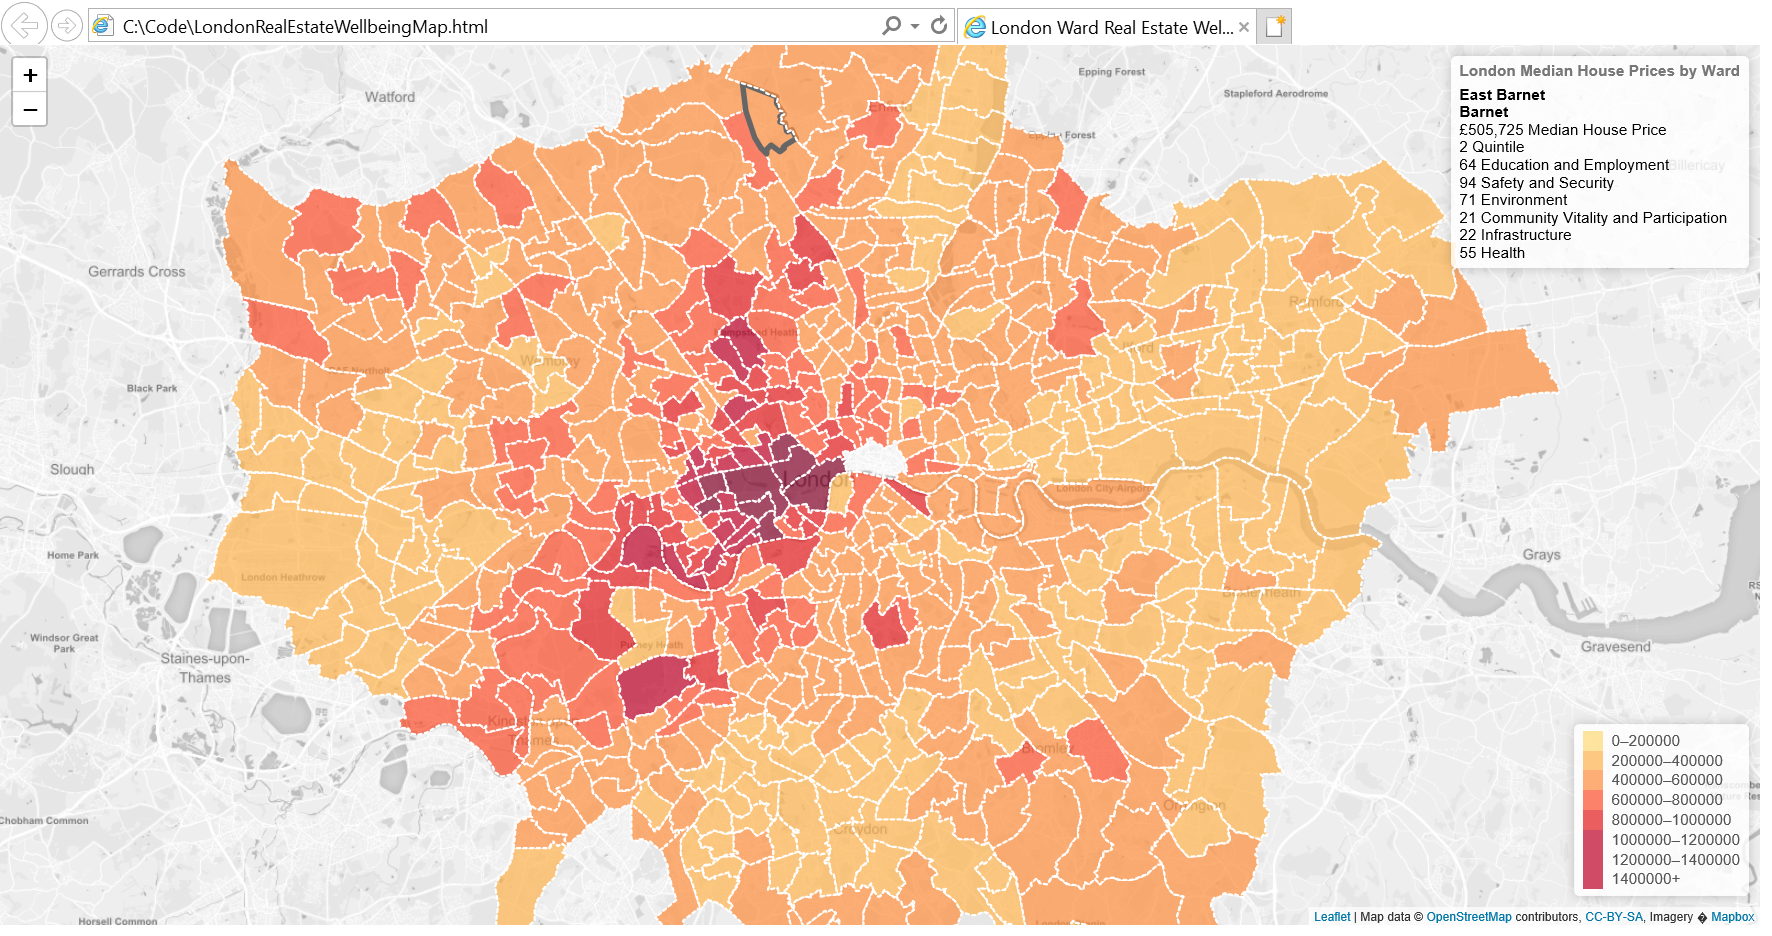
\includegraphics[scale=0.3]{figures/trailer_1}
\decoRule
\caption{Visualisation of median house prices by ward in London. Hovering over a particular ward will provide information on the well-being indices for that ward and the modelled median house prices and associated quintiles.}
\end{figure}

% Chapter Template

\chapter{State of the art} % Main chapter title

\label{ChapterX} % Change X to a consecutive number; for referencing this chapter elsewhere, use \ref{ChapterX}

%----------------------------------------------------------------------------------------
%	SECTION 1
%----------------------------------------------------------------------------------------

\section{Geospatial analysis in Data Science}

Maps are an increasingly popular way to visualise data where some form of geographic aspect is an important element of the analysis. The website London Mapping (\cite{LMap}) is a good example of the large amount of data analysis and visualisation taking place through the creation of various types of map for the city of London alone.

\begin{figure}[H]
\centering
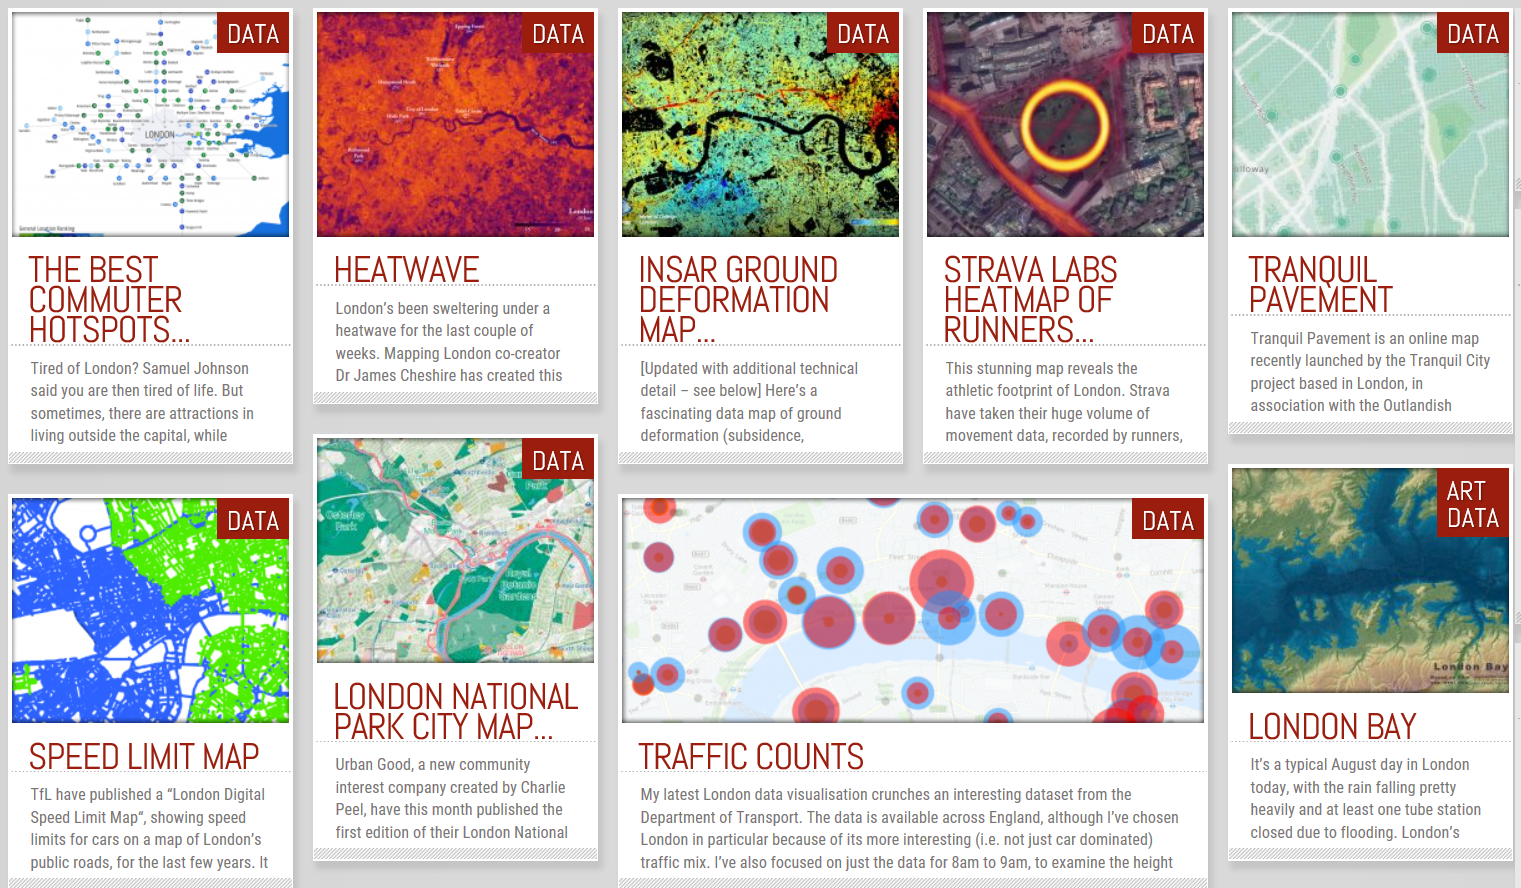
\includegraphics[scale=0.5]{figures/london_mapping}
\decoRule
\caption{An range of the maps exploring London on the Mapping London website. This website has been created by academics from the geography department at UCL and features a range of data-driven maps using various geospatial techniques.}
\end{figure}

There are several reasons why maps a a good choice for data visualisation which include:
\begin{itemize}
\item
They provide a real-world context for the data, helping the audience to understand the analysis
\item
They allow users to compare data over different areas or regions at a glance
\end{itemize}

Data Science techniques play an important role in the creation of this kind of visualisation. Most map visualisations represent locations through coordinate reference systems which represent locations. These locations can be specific locations represented by pairs of coordinates, most often (latitude, longitude), or areas which would be represented by polygons consisting of multiple coordinate pairs. Data Science techniques are required to design functions and algorithms to map, aggregate or disaggregate data between different types of geometry and different coordinate reference systems. 
	
%-----------------------------------
%	SUBSECTION 1
%-----------------------------------
\subsection{Point Maps}
One mapping technique often used in interactive visualisations would be a point map where specific instances of something are plotted as points in the geo-location in which they occur. This form of mapping would use a coordinate pair, often latitude and longditude but potentially an Ordnance Survey grid reference or other coordinate reference system. An example of this would be the Great British Public Toilet Map (\cite{rca14})

\begin{figure}[H]
\centering
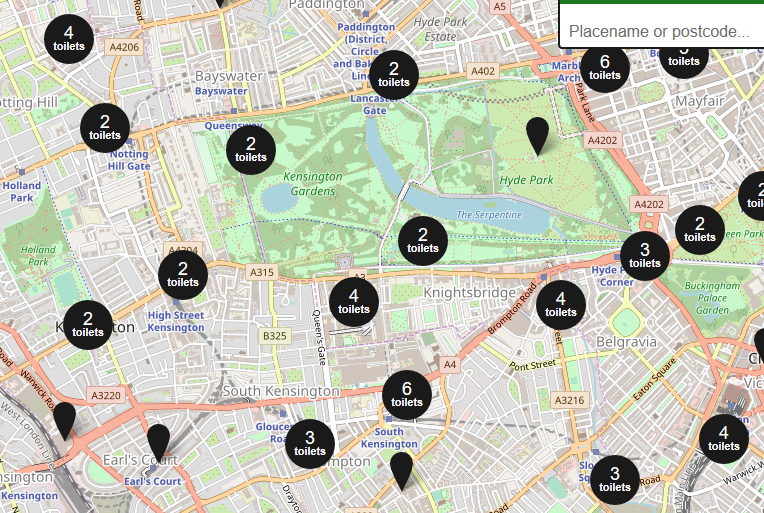
\includegraphics[scale=0.5]{figures/toilets_point}
\decoRule
\caption{An example of a point map - the Great British Public Toilet map created by the Royal College of Art in 2014 showing instances of public lavatories across the country.}
\end{figure}

%-----------------------------------
%	SUBSECTION 2
%-----------------------------------

\subsection{Choropleth Maps}
The city of Toronto is a good example of where an informative interactive well-being map has been created (\cite{toronto_2018}). On this map a user can click on an area and is presented with a panel showing the values for a number of measures.

\begin{figure}[H]
\centering
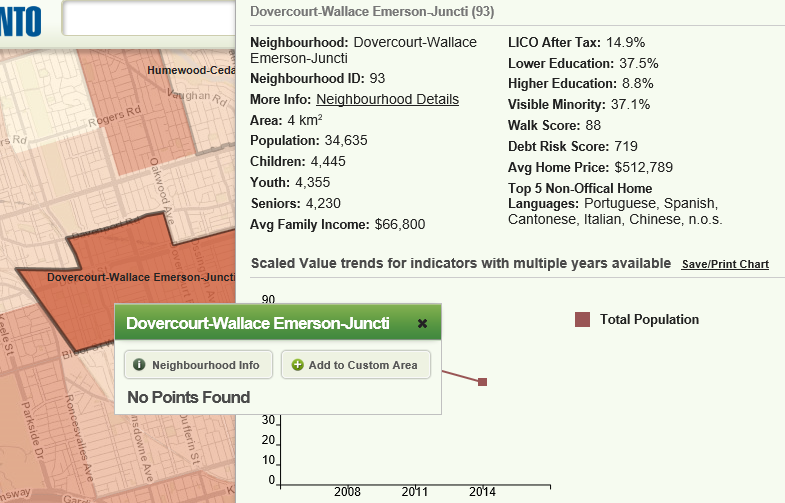
\includegraphics[scale=0.5]{figures/toronto_choropleth}
\decoRule
\caption{An example of a choropleth map - created by the City of Toronto to provide information about the neighbourhoods of urban Toronto.}
\end{figure}

The Toronto map uses a thematic mapping technique known as a Choropleth map, using shape files where polygons represent an area of space, in this instance neighbourhoods, with the colour of the polygon related to the value of the area in question.
This map is an excellent design example for this project as the geometries used, in this case neighbourhoods of Toronto, are of a similar geospatial representation to London Wards. The project map will be based on median house prices and hovering over an area will display the values of the well-being indicators and the projected values of the model.

%-----------------------------------
%	SUBSECTION 3
%-----------------------------------

\subsection{Heat Maps}
Real estate values have also been an area of interest for mapping. In recent times these visual displays of real estate value have often been created by the commercial sector, for example, UK property price maps created by the estate agent Zoopla (\cite{zoopla}). This is an example of a heat map.
Heat maps share similarities with Choropleth maps in that they assign a colour to an area based on the magnitude of a particular value. Where these two types of map differ is that heat maps assign colour to a cluster of connected points whereas for Choropleth maps, the colouration is based on a value for a polygon representing a given area, usually a administrative or political boundary.

\begin{figure}[H]
\centering
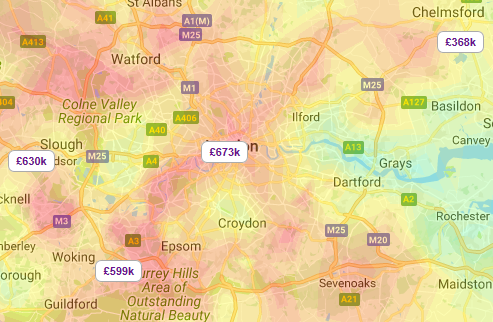
\includegraphics[scale=1]{figures/zoopla_heat}
\decoRule
\caption{An example of a heat map - a 2011 map created by the estate agents Zoopla to show UK average house prices.}
\end{figure}

%-----------------------------------
%	SUBSECTION 4
%-----------------------------------

\subsection{Network Maps}
An interesting alternative approach has been taken by (\cite{QAS16}) who have created a series of interactive maps using crowdsourced data and image processing techniques. The locations used in the maps created by Quercia et al. use specific locations represented by images and sound recordings rather than areas of space. Here, rather than using traditional spatial analysis techniques, the maps have been created using graphs which represent London as a network. The location of the images/sounds are the nodes and the routes between them form the vertices.

\begin{figure}[H]
\centering
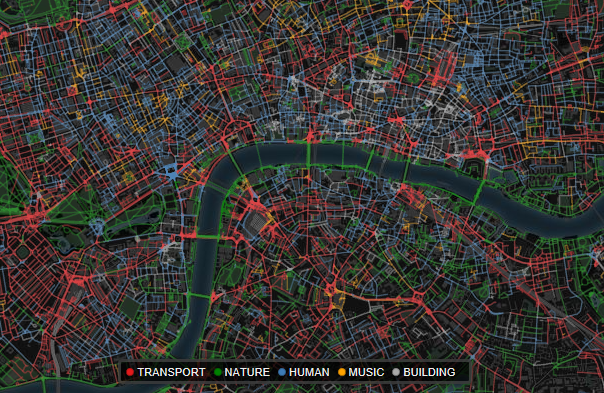
\includegraphics[scale=0.8]{figures/noise_network}
\decoRule
\caption{An example of a network map - created by Quercia, Aiello and Schifanello in 2016, this map categorises each road in London based on the primary type of noise heard in the location.}
\end{figure}


 
% Chapter Template

\chapter{Data Sources} % Main chapter title

\label{Chapter3} % Change X to a consecutive number; for referencing this chapter elsewhere, use \ref{ChapterX}

%----------------------------------------------------------------------------------------
%	SECTION 1
%----------------------------------------------------------------------------------------

\section{Datasets required to create the well-being indices}

To create the well-being indices the decision was made to use six indices each made up of three indicator datasets. For the purpose of the project, each index and indicator will be of equal weighting.
This approach is based upon other indices of well-being where data feeds into a set of between five and ten indices. 
Three examples of this type of index would be the Gross National Happiness index (\cite{GNH}), the OECD Better Life Initiative (\cite{BLI}) and the Canadian Index of Wellbeing (\cite{CIW}). 
The approach taken was to find three indicators that both represented each index and where the data could be retrieved or transformed to be analysed at ward level.

\begin{table}[H]
\caption{Indices and indicators used for the measurement of well-being for each London ward with data source and metric used}
\scalebox{0.4}{
\begin{tabular}{llll}
\toprule
Index                    & Indicators  & Source & Metric       \\
\midrule
\multirow{3}{*}{Education and Employment} & Average GCSE points & London datastore & Average GCSE capped point score \\
                         & Average Ofsted rating of schools & edubase @ gov.uk & Average Ofsted ratings of schools - most recent inspections (September 2018) \\
                         & Employment rates  & London datastore   & Rate of economically active individuals (2011)            \\
\hline
\multirow{3}{*}{Safety and Security}     & Crime rates - against the person  & London datastore & Number of recorded crimes (2017)\\
                         & Crime rates - other crime    & London datastore  & Number of recorded crimes (2017) \\
                         & Traffic injuries  & London datastore & Road collision numbers (2014) \\
\hline
\multirow{3}{*}{Environment}     & Air pollution & London datastore & Annual mean of Nitrogen Dioxide (NO2) and Particle emissions (PM10) (2011) \\
                         & Amount of greenspace  & London datastore    & Percentage of ward area which is greenspace (2011)  \\
                         & Access to nature & London datastore & Percentage of residential households with access to at least one open space (2011)\\
\hline
\multirow{3}{*}{Community Vitality and Participation} & Access to cultural space  & Foursquare & Number of cultural venues in ward (August 2018)\\
                         & Amount of bars and restaurants   & Foursquare  & Number of bars and restaurants in ward (August 2018)\\
                         & Election turnout & London datastore  & Percentage of residents voting in 2016 London election\\
\hline
\multirow{3}{*}{Infrastructure} & Access to public transport & London datastore & Transport for London Public Transport Accessibilty Levels (2015) \\
                         & Average journey times   & gov.uk  & The mean percentage value of those within an hour's travel by public transport or walking of an area of 100, 500 and 500 jobs (2014)\\
                         & Population density & London datastore & Persons per square km (2013)\\
\hline
\multirow{3}{*}{Health}  & Life expectancy & London datastore & Life expectancy at birth (2013) \\
                         & Childhood obesity   & London datastore   & Prevalence of obese children at age 11 (2013)  \\
                         & Illness preventing employment & gov.uk  &  Comparative illness and disability ratio from English Indices of Deprivation (2015)\\
\bottomrule\\              
\end{tabular}
}
\end{table}

Access to open space definition \footnote{\url{https://data.london.gov.uk/dataset/access-public-open-space-and-nature-ward}}

Access to public transport definition \footnote{\url{https://data.london.gov.uk/dataset/public-transport-accessibility-levels}}

Illness preventing employment definition  \footnote{\url{https://www.gov.uk/government/statistics/english-indices-of-deprivation-2015}}

%----------------------------------------------------------------------------------------
%	SECTION 2
%----------------------------------------------------------------------------------------

\section{Static data files}

The majority of data sets are either csv or Excel files which are accessed directly via a url by the data importer application. These sources are primarily from the websites of public bodies. The data importer application makes use of the pandas module within Python to support the importing and cleaning process within a series of dataframe objects.

%-----------------------------------
%	SUBSECTION 1
%-----------------------------------
\subsection{London datastore}

The Greater London Authority Datastore (\cite{GLA}) was the primary source of data for the project with significant amounts of data relating to various London metrics available. The fact that much of the data contained on the website was available at ward level was key in being able to piece together the indices.


%-----------------------------------
%	SUBSECTION 2
%-----------------------------------

\subsection{gov.uk}

Used for Ofsted ratings for schools, average journey times and illness affecting employment, the gov.uk website contains a varied range of datasets. 
Three key datasets used from this source are Edubase schools information for Ofsted ratings, 2014 Department for Transport journey time statistics and 2015 English Indices of deprivation.
Without the London focus of the GLA datastore, information on gov.uk is often harder to locate and in many cases is at a higher level of aggregation than required with most information at borough or national level.

%-----------------------------------
%	SUBSECTION 4
%-----------------------------------

\subsection{esri}

Data for average journey times and illness affecting employment was obtained at lower super output area, a lower level of aggregation than ward. The different geographical level use in the two datasets created the need for a mapping. The open data section of esri's ArcGIS website (\cite{ArcGIS}) offered this mapping document in csv format which could be incorporated into the data import software to allow an arithmetic mean to be determined at ward level.


%----------------------------------------------------------------------------------------
%	SECTION 3
%----------------------------------------------------------------------------------------

\section{APIs}

A subset of London data is also available via various APIs. For transport information Transport for London have extensive APIs available, unfortunately none of these were able to provide any of the datasets required for the project, though other formats offered by TFL were used. The use of APIs became focussed on collecting information on venues to obtain the data for the 'community vitality' and 'access to cultural spaces' datasets. For this data Foursquare was the primary candidate with venue information available with no cost implications. 

%-----------------------------------
%	SUBSECTION 1
%-----------------------------------

\subsection{Foursquare}

Foursquare is a social media platform based on location intelligence. The platform has information on more than 105 million locations mapped worldwide and over 50 million users per month. (\cite{foursquare}). With the extensive database of venues with location information, Foursquare could be used to look at two of the indicators which feed into the Community Vitality and Participation index:
\begin{itemize}
\item Access to cultural spaces
\item Popularity of bars and restaurants
\end{itemize}
To measure these two indicators, Foursquare's venue API can be used to return list of venues within a radius of a specific point provided in latitude and longditude.
By using the three venue types, "culture", "food" and "nightlife", a list of venues fitting those types can be captured via the API. In the implementation phase, the list of venues containing the point location of the venues can be mapped to the relevant ward and numbers aggregated to give an indicator of volume with which to measure this category.


%-----------------------------------
%	SUBSECTION 2
%-----------------------------------

\subsection{Google Maps}
The places API from Google Maps was queried and code written to extract venue data. However, after obtaining some basic search results it was decided that Google's pricing policy and rate limits made this data source unfeasible for the scope of the project.

%----------------------------------------------------------------------------------------
%	SECTION 3
%----------------------------------------------------------------------------------------

\section{Shape Files}

For choropleth mapping, shape files are needed to visualise the polygon shapes which define adminstrative or political boundaries. Shape files usually consist of properties of the shape such as name and size along with a geometry feature which defines the boundaries of a given shape via the coordinates of their vertices. For this project, the relevant shapefile is key to creating the final interactive map and will also be use to visualise the data and support the model building process.  

%-----------------------------------
%	SUBSECTION 1
%-----------------------------------
\subsection{London Ward shapefile}

The key shapefile for the project is taken from the London datastore and provides the polygon geometry of the London wards. This is a .shp file where the point coordinates which make up the polygon for each ward are in the Ordnance Survey grid reference cooridnate reference system. With point geometries more often listed in latitude and longditude, there will need to be some reprojection of coordinates to enable certain datasets to match with the shapefile.

%----------------------------------------------------------------------------------------
%	SECTION 4
%----------------------------------------------------------------------------------------

\section{Data availability issues}

In part thanks to the Greater London Authority’s Datastore, a wealth of information is available at London Ward level. Combining this with information from the Foursquare API and Department for Education schools data provided a significant body of information in which to model London as a multiple dataset.
Data availability was such that datasets for each of the indicators feeding into the six indices were available and it was not necessary to use substitute indicators that differed significantly from those originally planned. 

%-----------------------------------
%	SUBSECTION 1
%-----------------------------------
\subsection{Timeliness}

Some of the datasets related to different years, often linked to census years and administrative or electoral changes.
Wherever possible the most recent data has been used to synchronise as closely as possible with the 2017 data used for the median house price data. For example, Emission data is from 2011 as this is the most recently published at ward level. The London Air Quality daily feed run by King’s College does not have enough coverage to sufficiently differentiate over 600 wards. Ideally this data would have been from the same year as the house price information.

%-----------------------------------
%	SUBSECTION 2
%-----------------------------------

\subsection{Boundary changes}
Ward boundaries were re-drawn in three London Boroughs in 2014 meaning that a function had to be written that, for data pre-dating 2014, would map old ward codes to the new ward that contained the largest section of the newly defined area. Newer data would also have been helpful here but the commonality of area between the old and new codes in the mapping should ensure that the data is representative of the new area.

%-----------------------------------
%	SUBSECTION 3
%-----------------------------------
\subsection{API rate limits}

API limits and costs imposed limits on the depth of information that could be obtained from these sources. Whilst I was able to obtain the necessary Foursquare venue and venue location information, venue ratings and check-ins were subject to stringent daily limits which meant that obtaining this information would have taken weeks of daily iterations or significant costs neither of which were feasible for this project. I investigated the possibility of using Google Places API but the new pricing model introduced this year also made this unfeasible. In a commercial setting it may be possible to increase the amount of data that can be obtained from some of the APIs.

% Chapter Template

\chapter{Design} % Main chapter title

\label{Chapter4} % Change X to a consecutive number; for referencing this chapter elsewhere, use \ref{ChapterX}

%----------------------------------------------------------------------------------------
%	SECTION 1
%----------------------------------------------------------------------------------------

\section{Architecture of the specification}

%-----------------------------------
%	SUBSECTION 1
%-----------------------------------
\subsection{Archictecture diagram}

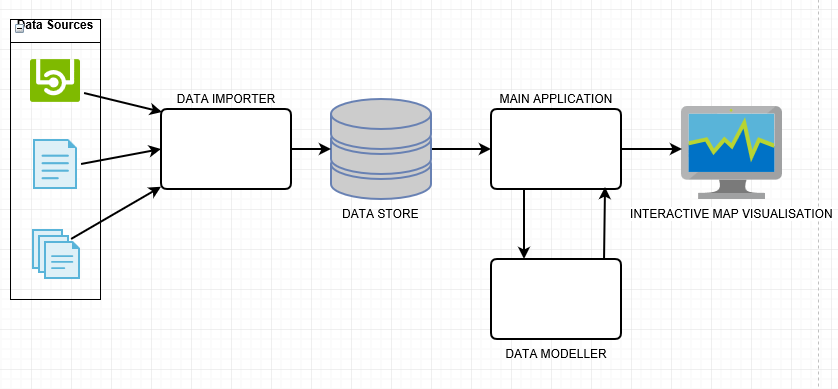
\includegraphics[scale=0.75]{figures/Software_Architecture} % Code example


%-----------------------------------
%	SUBSECTION 2
%-----------------------------------

\subsection{Architecture choices}
For this project two main technologies are being used, Python and Javascript. The majority of the software code has been written in Python, specifically for the data import processes, for the main application which runs the analysis and geocoding and the data modelling component. Python was chosen for these components for a number of factors. Firstly for the data importer, Python has excellent capabilities for data processing allowing the data to be collected and cleaned leveraging the Pandas module. For the main application, Python's geocoding and spatial capabilites were important factors in the choice. The ability to import shape files and reproject coordinate systems leveraging Geopandas and Shapely allowed more flexibility in which datasets were suitable for the project and the option to export to GeoJSON format facilitated the data visualisation.
For the visualisation stages Javascript embedded in a html file was chosen. For this final component of the project Javascript was preferred to Python due to the interactive element required on the map. With the aid of the Leaflet.js package in Javascript I was able to make use of more map features to present any end users with a more complete user experience.


%----------------------------------------------------------------------------------------
%	SECTION 2
%----------------------------------------------------------------------------------------

\section{Components}

The software architecture design for the project has been created with the aim of being able to isolate individual elements in the interest of performance. The system is not dependent on processing a live data feed so it is important that the component that imports the data does not have to run everytime a user would wish to access the interactive map visualisation. The design means that each component can be modified and without affecting the other parts.  


%-----------------------------------
%	SUBSECTION 1
%-----------------------------------
\subsection{Data inputs}
The data input layer is the base layer of the system. This consists of several different types of input including API feeds from the Foursquare platform, csv files collected directly from urls and other data files which have been pre-collected and loaded into the data store. This layer is the most likely to change moving forward as new and updated data sources are published or become available in alternative formats.

%-----------------------------------
%	SUBSECTION 2
%-----------------------------------

\subsection{Data importer}
The data importer software is written in Python and is designed as a series of functions. Each function imports one of the required datasets. Setting these up as seperate functions gives the option to run imports individually. This is an important requirement of the system as certain imports take a considerable amount of time. The iterative nature of the API imports combined with daily rate limits mean that it is only feasible to run the API imports from Foursquare on at most a daily basis. As the system is not reliant on a live feed, the data import software could be run as an overnight batch process. 

%-----------------------------------
%	SUBSECTION 3
%-----------------------------------

\subsection{Data store}
The data store is central to the architecture to safeguard performance levels. As the data imports are best suited to a batch process, the cleaned data files should be stored in the data store for the main application software to run efficiently. The data store is also used for any pre-collected data which cannot be collected directly from a url or API. This imports the data for the 18 base indicators which create the 6 well-being domains.

%-----------------------------------
%	SUBSECTION 4
%-----------------------------------

\subsection{Main application}
The main application software performs a variety of tasks and is written in Python. The first task that the software performs is to take the data that has been imported for the 18 base indicators from the data store. The main application then performs any data manipulation and applies a set of geocoding and spatial functions to standardise the data into a format where everything is aggregated for London Ward geometry. Having standardised, the software then creates the 6 well-being domains using functions drawing on Principal Component Analysis and mean calculation functions which also normalise the data to ensure that each score is between 0 and 100.
These 6 domains are then combined with data showing median house prices and the related quintiles and passed through the regression and classification models chosen through the data modeller component. The final task performed by this component is to create a geoJSON file including the well-being domain scores, median house price information, spatial data and predicted regression and classification values. This file contains the data used in the visualisation.

%-----------------------------------
%	SUBSECTION 5
%-----------------------------------

\subsection{Data modeller}


%-----------------------------------
%	SUBSECTION 5
%-----------------------------------

\subsection{Interactive map}
The final component of the software architecture is the interactive map which is built in javascript and html. This component builds a framework for the map using tiles from the MapBox service. A javascript function then takes the geoJSON file and add this as a layer to the map. This part of the architecture can be seen as the user front end as the visualisation allows users to hover over each ward to see the scores, actuals and predictions along with features such as a zoom facility. 
% Chapter Template

\chapter{Implementation} % Main chapter title

\label{Chapter5} % Change X to a consecutive number; for referencing this chapter elsewhere, use \ref{ChapterX}

%----------------------------------------------------------------------------------------
%	SECTION 1
%----------------------------------------------------------------------------------------

\section{Data collection and cleaning}

The key foundation of the project was being able to collect the data that would allow the creation of the well-being domain scores. Collecting the required data and shaping it into the formats that were needed was, in places, one of the most challenging aspects of the project and the one that required the largest proportion of time. This part of the project presented several challenges that needed to be overcome.

%-----------------------------------
%	SUBSECTION 1
%-----------------------------------
\subsection{Collection of data files}

For ward level data, the Greater London Authority's datastore is a primary data source. A significant proportion of the data for the creating of the well-being indicators could be accessed via this source. 

%-----------------------------------
%	SUBSECTION 2
%-----------------------------------

\subsection{Collection from APIs}

The API that was key to the success of the project was that of social media platform Foursquare. To represent community vitality, the aim was to create a measure for the restaurants and bars in each ward. Foursquare is a platform based around venue information so holds the information required for this measure. Foursquare also holds information on cultural venues. Therefore the measure of 'Access to Cultural Space' could also be obtained from this platform.
To use the API to obtain venue information you are required to search for venues within a specified radius of a certain point, given in latitude and longditude. The challenge with Foursquare was the the API rate limits which limits each search to a maximum of 49 searches. There are also daily and monthly rate limits to stay within.
To obtain results of all bars, restaurants and cultural venues accross Greater London with these limits an iterative algorithm had to be created which could travel accross London by latitude and longditude, taking in small enough areas so as to not exceed 49 results a time. To achieve this, I created a latitude and longditude bounding box around London and created a nested loop iteration of 50 points of latitude and 50 points of longditude. The areas created by this had some overlap so as not to have missing areas of the capital. With a counter to check if the search limit of 49 venues was exceeded, this search algorithm put the list of venues into a pandas dataframe and de-duplicated for where areas had ovelapped.

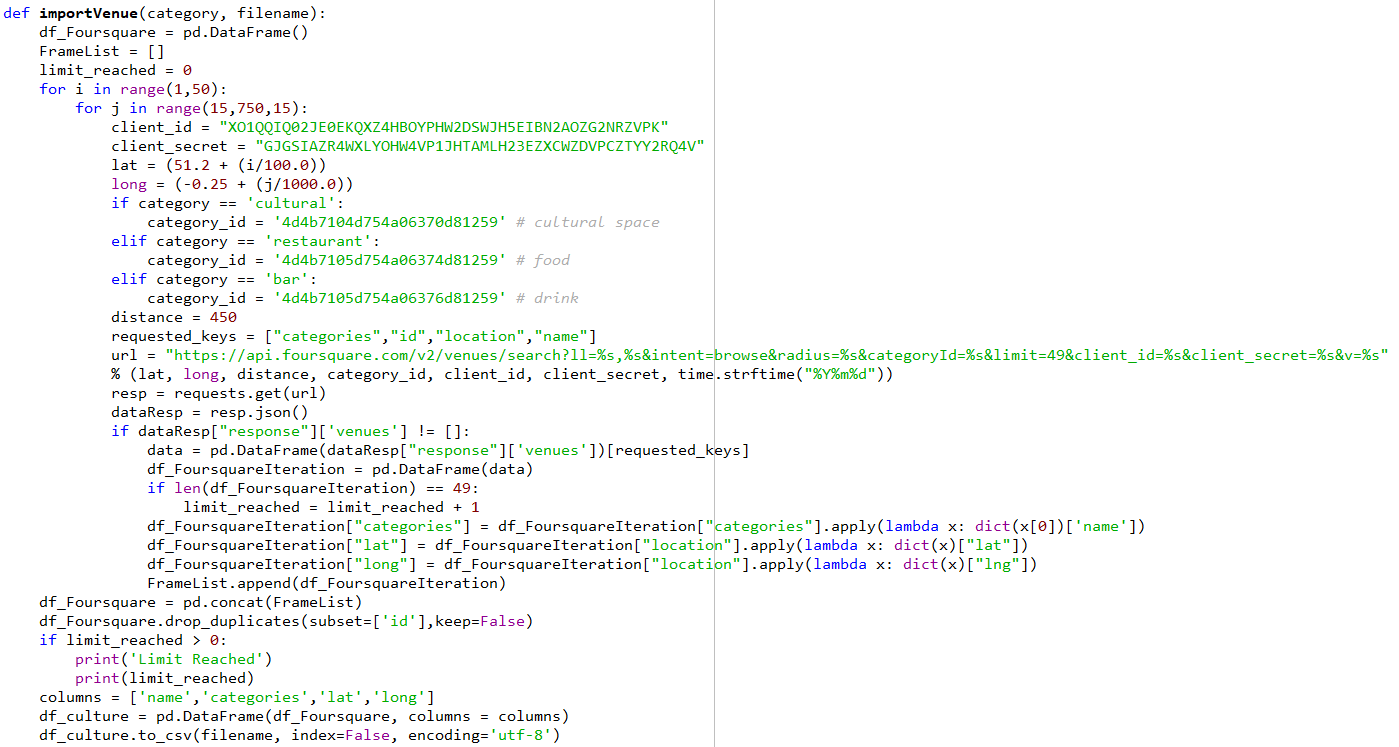
\includegraphics[scale=0.75]{figures/API_import} % Code example

Because of the rate limits, running the algorithm for such a large area could only be done on a daily basis.

%----------------------------------------------------------------------------------------
%	SECTION 2
%----------------------------------------------------------------------------------------

\section{Well-being domain scores}

The motivation for creating composite domain scores 6 different measures of well-being was two-fold. Firstly creating a score for each domain over a pre-defined scale would allow users of the front-end interactive map compare scores accross wards and give those scores some contextual meaning and significance. With 6 domains rather than the original 18 datasets, the amount of information presented to the user would not be too large to prevent a non-technical audience from interpreting the information on the map. The second reason for creating the domain indicators was to help to try and create an interpretable model rather than one requiring significant dimension reduction. Whilst some less interpretable models will be tested to validate the quality of the quintile classification model, ideally the project and the user front end should allow us to draw some conclusions about any link between well-being and median house prices in London.

For each domain three appropriate datasets were chosen and then reduced to give a single score for each ward. The 3 datasets for each domain were standardised using a function in Python and those which related to a negative indicator such as emissions or crime were mutliplied by a value of -1. Using this technique of standardisation gave equal weighting to each of the three indicators. Because of the equal weighting given to each indicator, these can be seen as substitutable within the context of the domain which is a important factor in the choice of technique used to reduce the indicators to a score. With indicators that can be assumed to be substitutable suitable techniques would include Principal Component Analysis (PCA) and an arithmetic mean
?INSERT REFERENCE TO PAPER BY ITALIAN ACADEMICS?
For the 6 domains, a mixture of the two techniques have been used. For those domains where the 3 indicators have a relatively high correlation ?ABOVE WHAT? the first Principal Component has been used to try and extract the largest amount of variance within the three indicators. Where the indicators for a domain have low levels of correlation for at least one of the three datasets, the arithmetic mean has been used. This approach gives us three domains which use PCA and three which use the mean.
?INSERT COV MATRICES AND TECHNIQUES FOR EACH DOMAIN?
This approach tries to maximise the information contained in all of the datasets.
To create an interpretable and comparable score for each domain the resulting single scores have been normalised and then rescaled to be between 0 and 100, this is the score that is presented in the user front end.


%----------------------------------------------------------------------------------------
%	SECTION 3
%----------------------------------------------------------------------------------------

\section{London house prices as a regression problem}

London is known for having very high real estate values but we can see from the map below that there are specific wards, particularly in the western central area, where median house prices are significantly above the Greater London area as a whole.

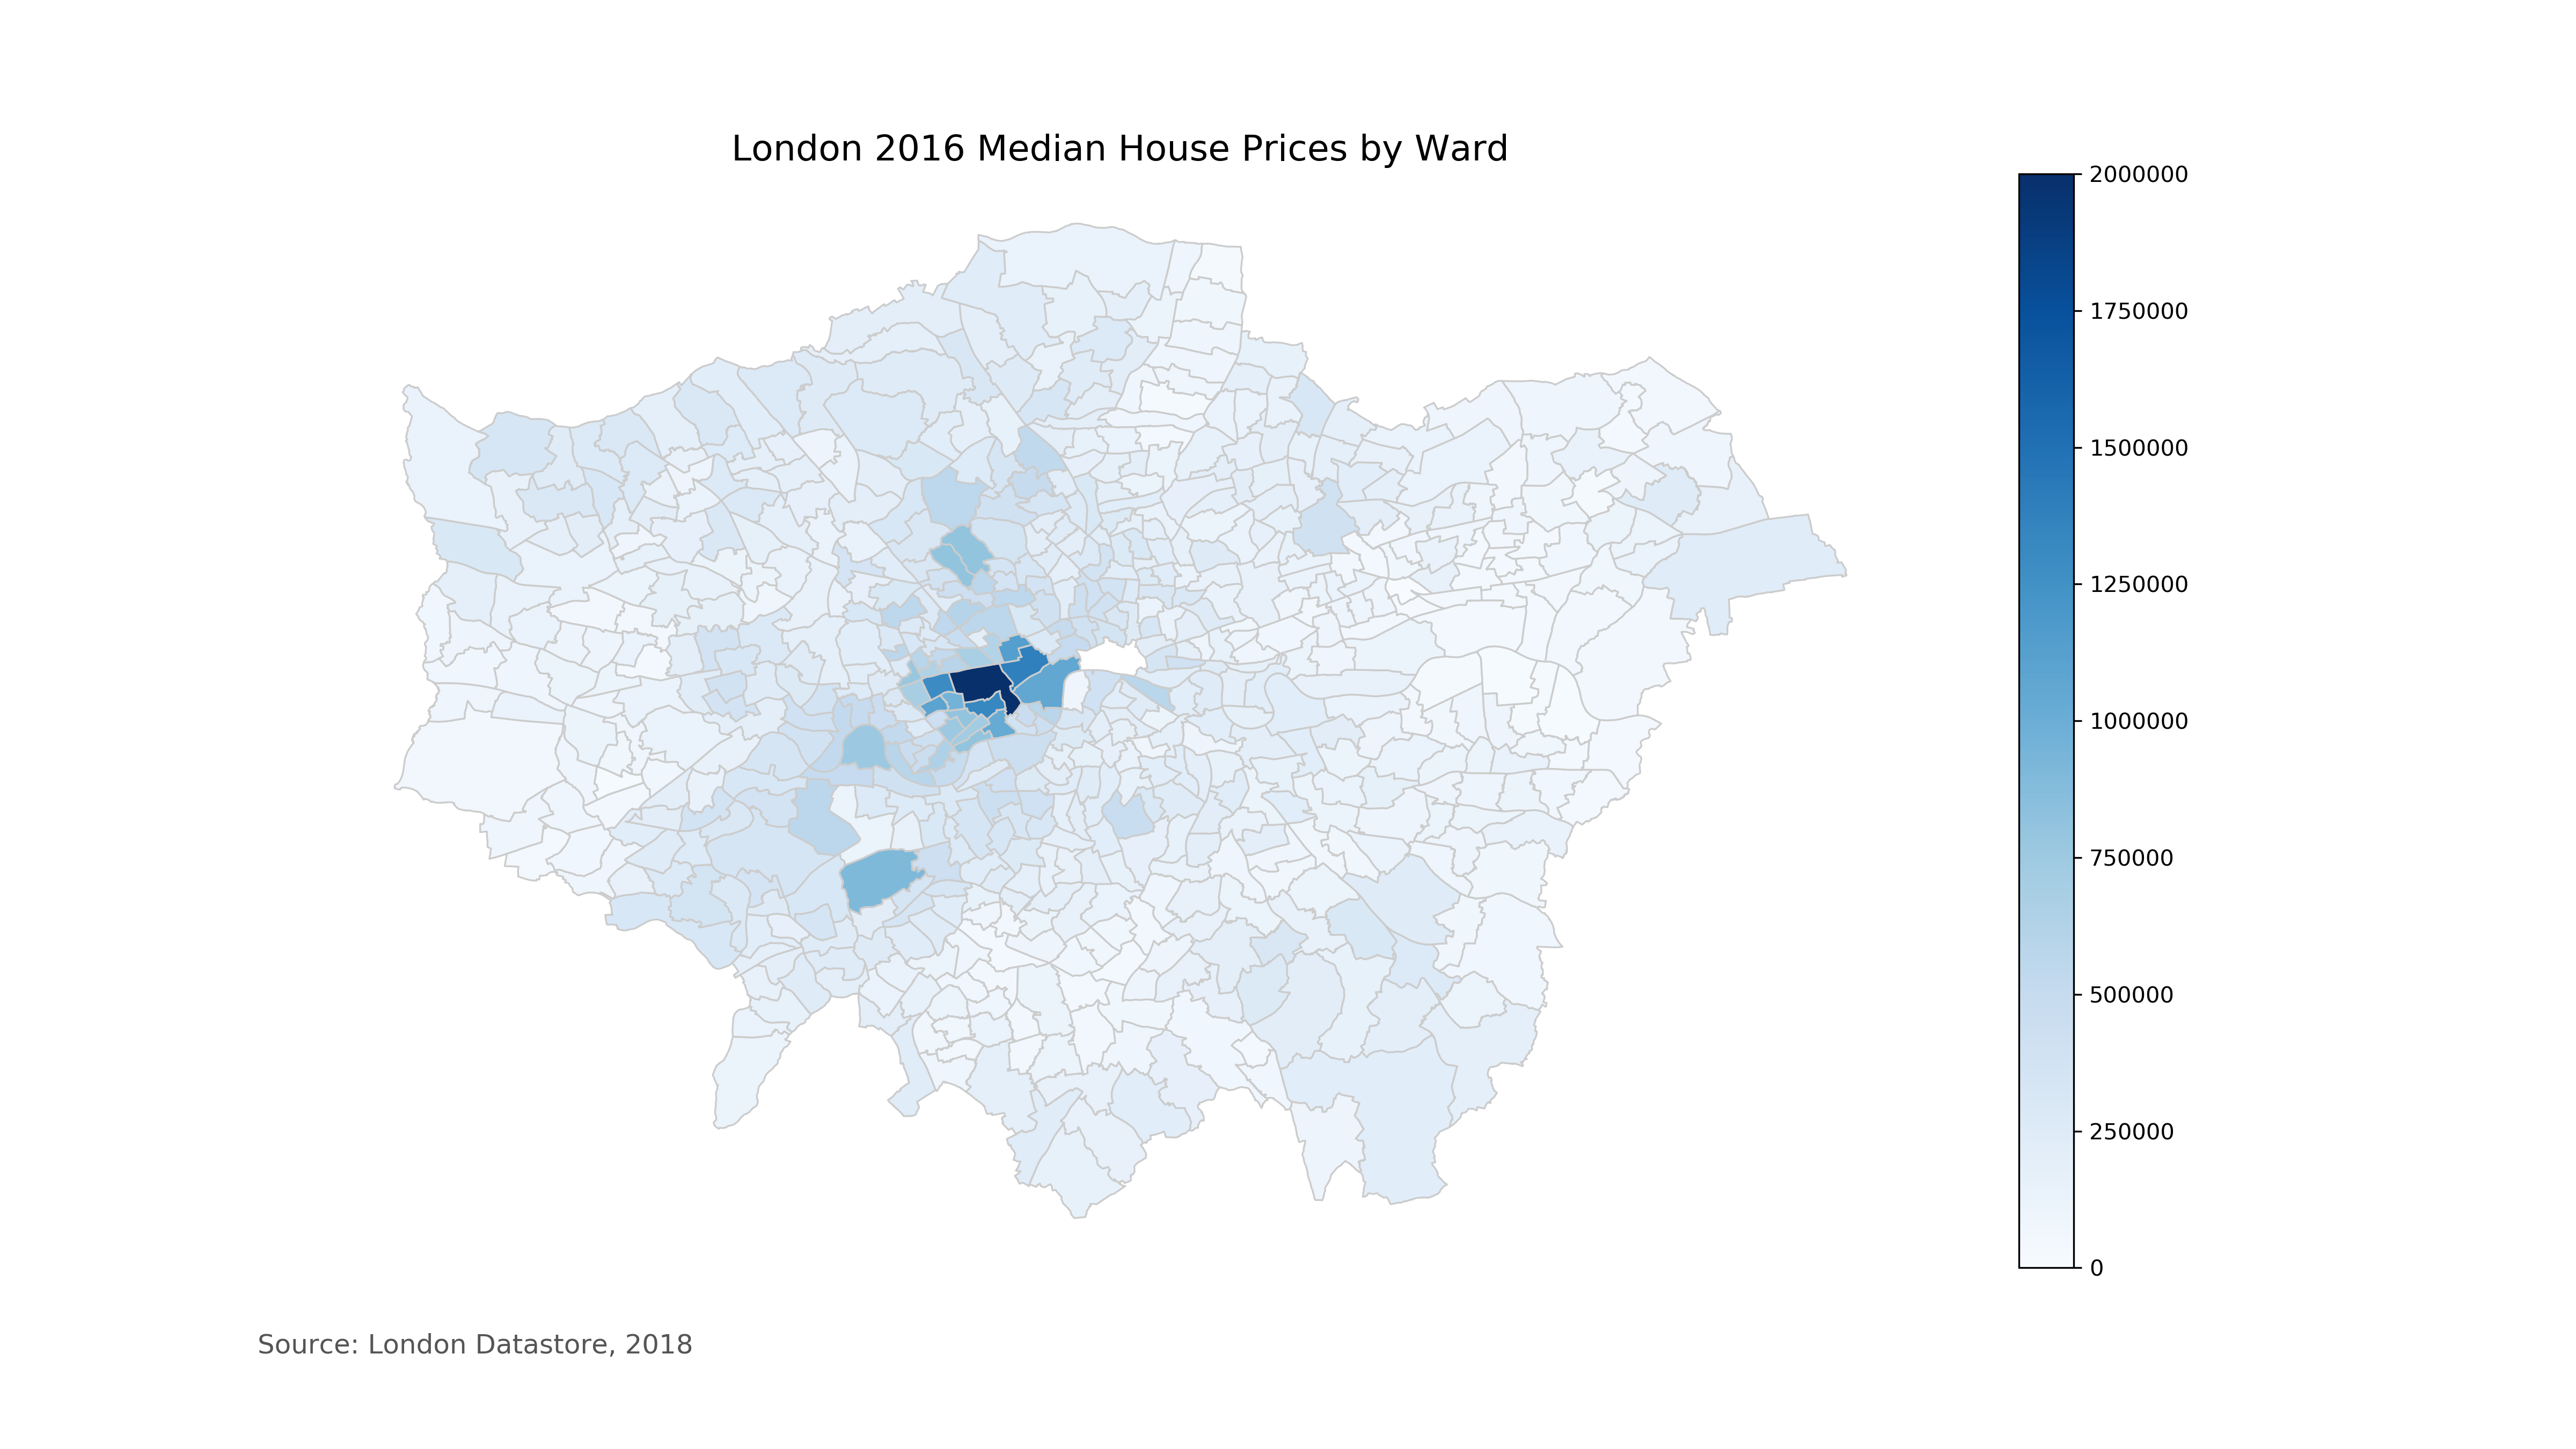
\includegraphics[scale=0.4]{figures/HPMedian} % Choropleth of median house prices

The choropleth map would suggest a high number of wards fall at the lower end of the range of median house prices with a small number with significantly high prices. From the pairwise plot below, the shape of the histogram of median house prices by ward would suggest that a power law may best describe the distribution.

? FIT POWERLAW TO MEDIAN HOUSE PRICES ?

For the domain scores, the histograms show most of the six as being at least close to a normal distribution. This is less clear in the case of the Safety and Security and Community Vitality and Participation domains with Safety and Security showing a large number of high values and Community Vitality and Participation showing many low scores. This can be attributed to a small number of wards where crime is high and that wards in central London have much greater access to both cultural and social spaces as indicated on the maps below. In both cases, a power law may best describe these distributions.

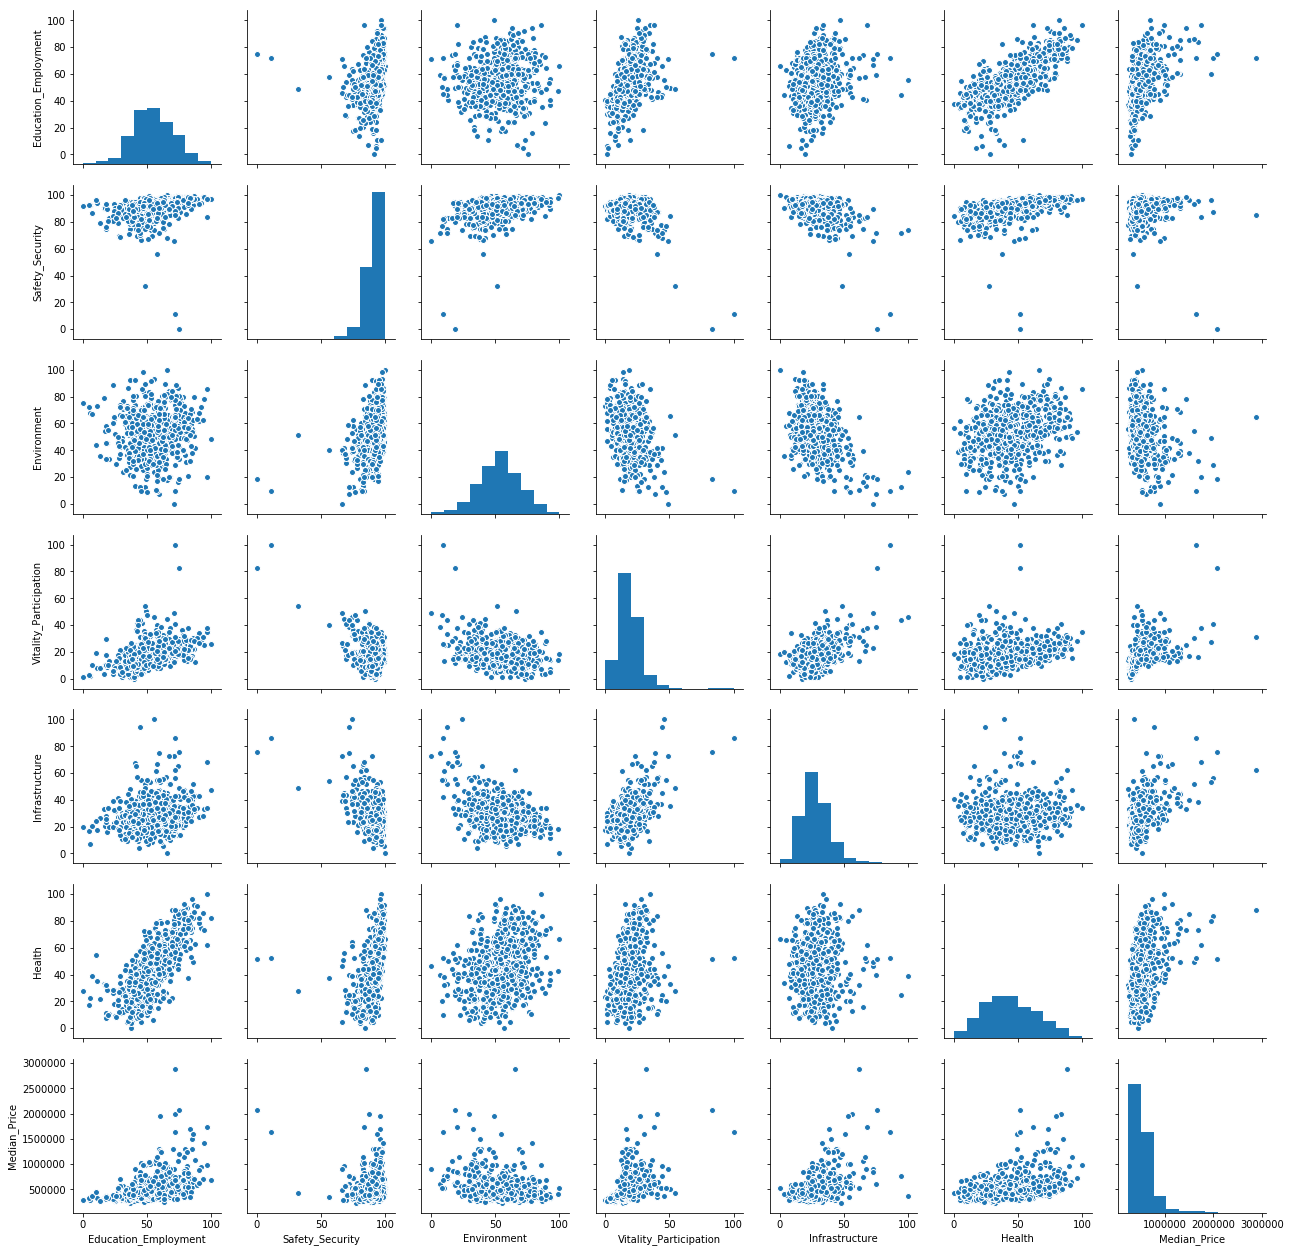
\includegraphics[scale=0.3]{figures/pairplot} % Pair-wise plot with median prices

This is less clear in the case of the Safety and Security and Community Vitality and Participation domains with Safety and Security showing a large number of high values and Community Vitality and Participation showing many low scores. This can be attributed to a small number of wards where crime is high and that wards in central London have much greater access to both cultural and social spaces as indicated on the maps below. In both cases, a power law may best describe these distributions.

Correlations

?INSERT MAPS OF EACH DOMAIN?

To begin the task of trying to model the median house prices from the well-being indicators, a simple multiple linear regression model was used with all six domains as predictors. The results show that this model explains less than half the variance with an R sq score of 0.39. There is enough to suggest that some form of linear model may provide a reasonable model of this problem.
To validate the model K-fold cross validation was used with k=7 with accuracy scores and mean squared errors average accross the seven iterations.

? STATSMODEL ?

Next a polynomial model was tried with degree two. This model explained almost none of the variance with an R sq value of very close to 0. The mean squared error also increased dramatically. The polynomial model does not seem to be a strong candidate for solving the problem.

The next models involved some feature reduction based on the p values of the domains in the original linear model. This meant that first Education and Employment were removed and then Community Vitality and Participation. This resulted in a small improvement in the model fit but little improvement in the MSE. 

With the median house price distribution suggesting a power law, a log transformation was performed on the data to try and linearise it with the linear regression model then re-run. This transformation dramatically increased the R sq value of the model, to 0.64, an increase of 0.25 from the equivalent model without the transformation. The model run on the log transformed data explains an additional 25 percent of the variance within the model. The exponent of the MSE is also a substantial reduction. This returned the following model:

?[insert model equation]?

As the best performing regression model this will be used for prediction in the final visulisation.

When the predictions were given the inverse transformation and validated against the actual values, the majority of wards showed that this model had good predictive capability although there were a handful of wards where the prediction had a signifcant error margin. The wards with significant errors tended to be those which had a much higher or lower score in a particular domain as compared to the neighbouring areas.

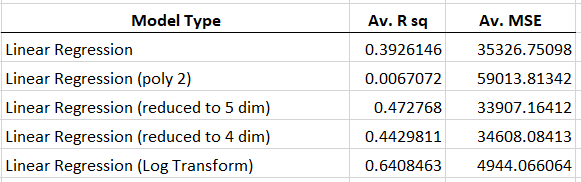
\includegraphics[scale=1]{figures/regression_results} % Regression results


%----------------------------------------------------------------------------------------
%	SECTION 4
%----------------------------------------------------------------------------------------

\section{London house prices as a classification problem}

The choropleth map below shows a different picture of London house prices being based on quintiles rather than monetary values, here the fifth quintile covers a larger range of values than the other quintiles due to the extremely expensive areas such as Knightsbridge and Belgravia where the median house price reaches over £2.8 million, 10 times as much as North End ward in Bexley.

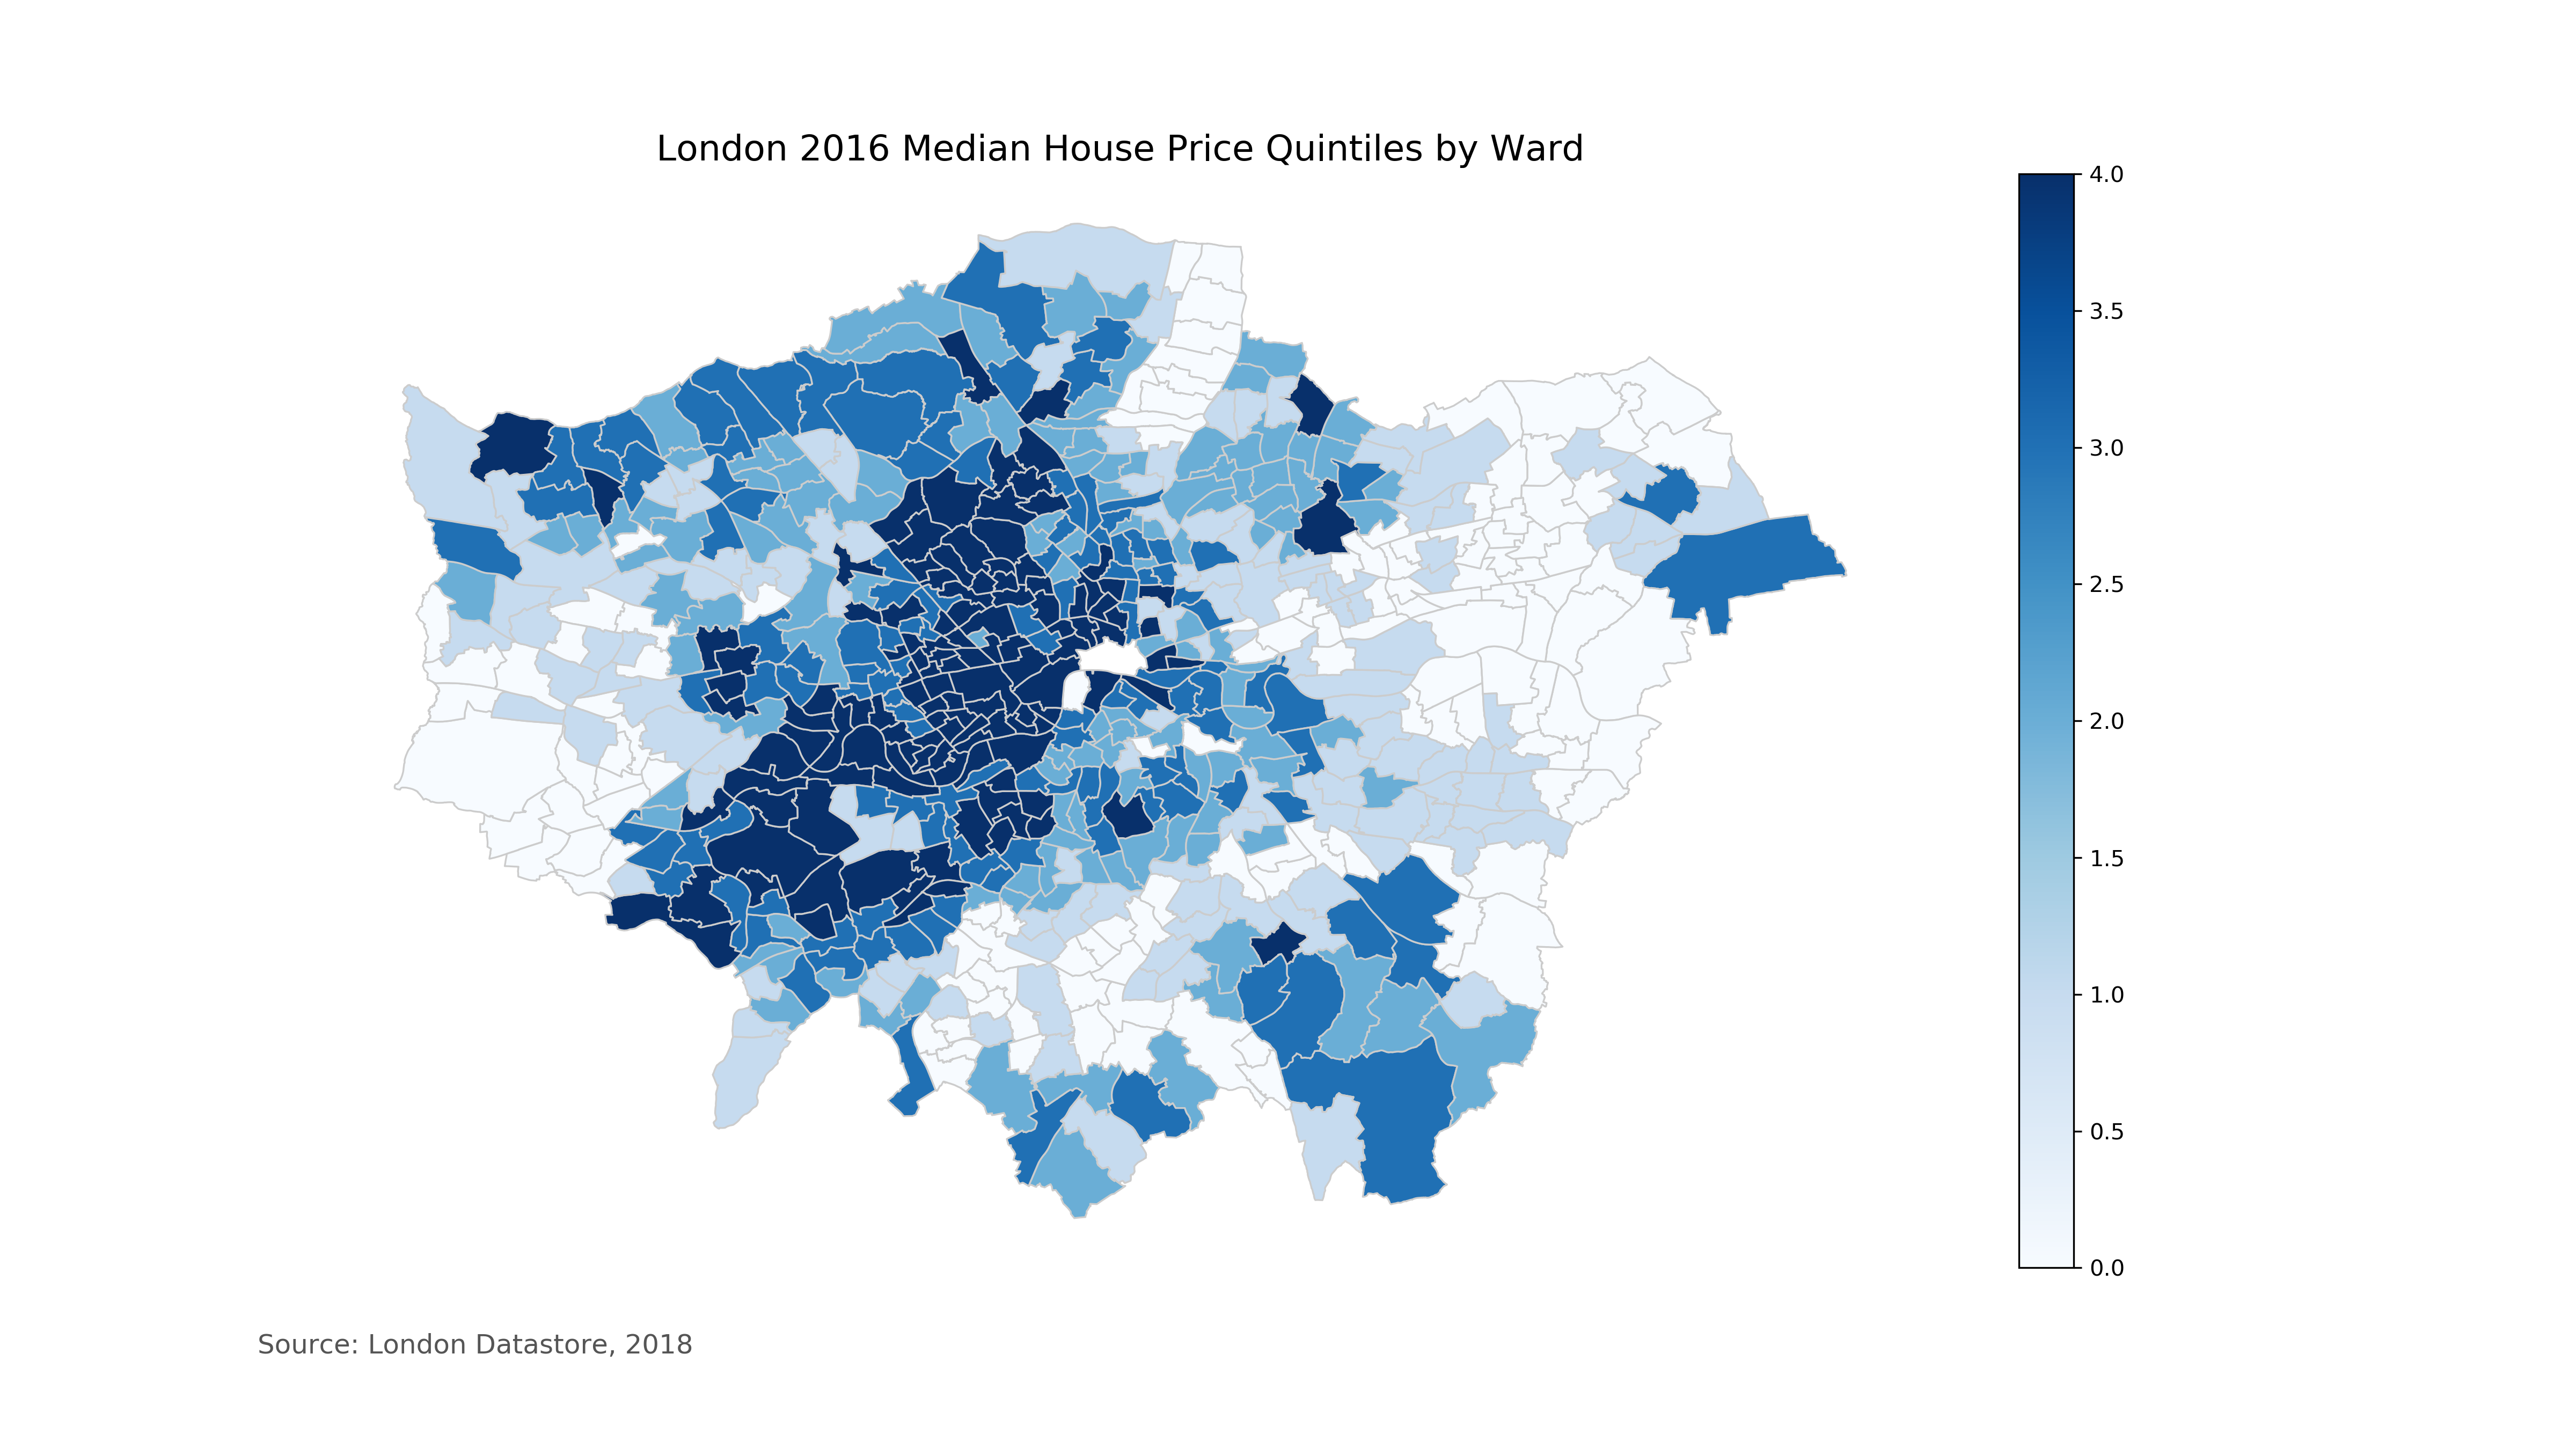
\includegraphics[scale=0.4]{figures/HPQuintile} % Choropleth of Median house prices by quintile

? BOXPLOT WITH QUINTILES ?

For the classification problem the aim was to try to find a model that has both a good fit and high interpretability. However, models that often have high accuracy but low interpretability such as support vector machines and neural networks were also used to both discover and validate the best classification model for the problem.

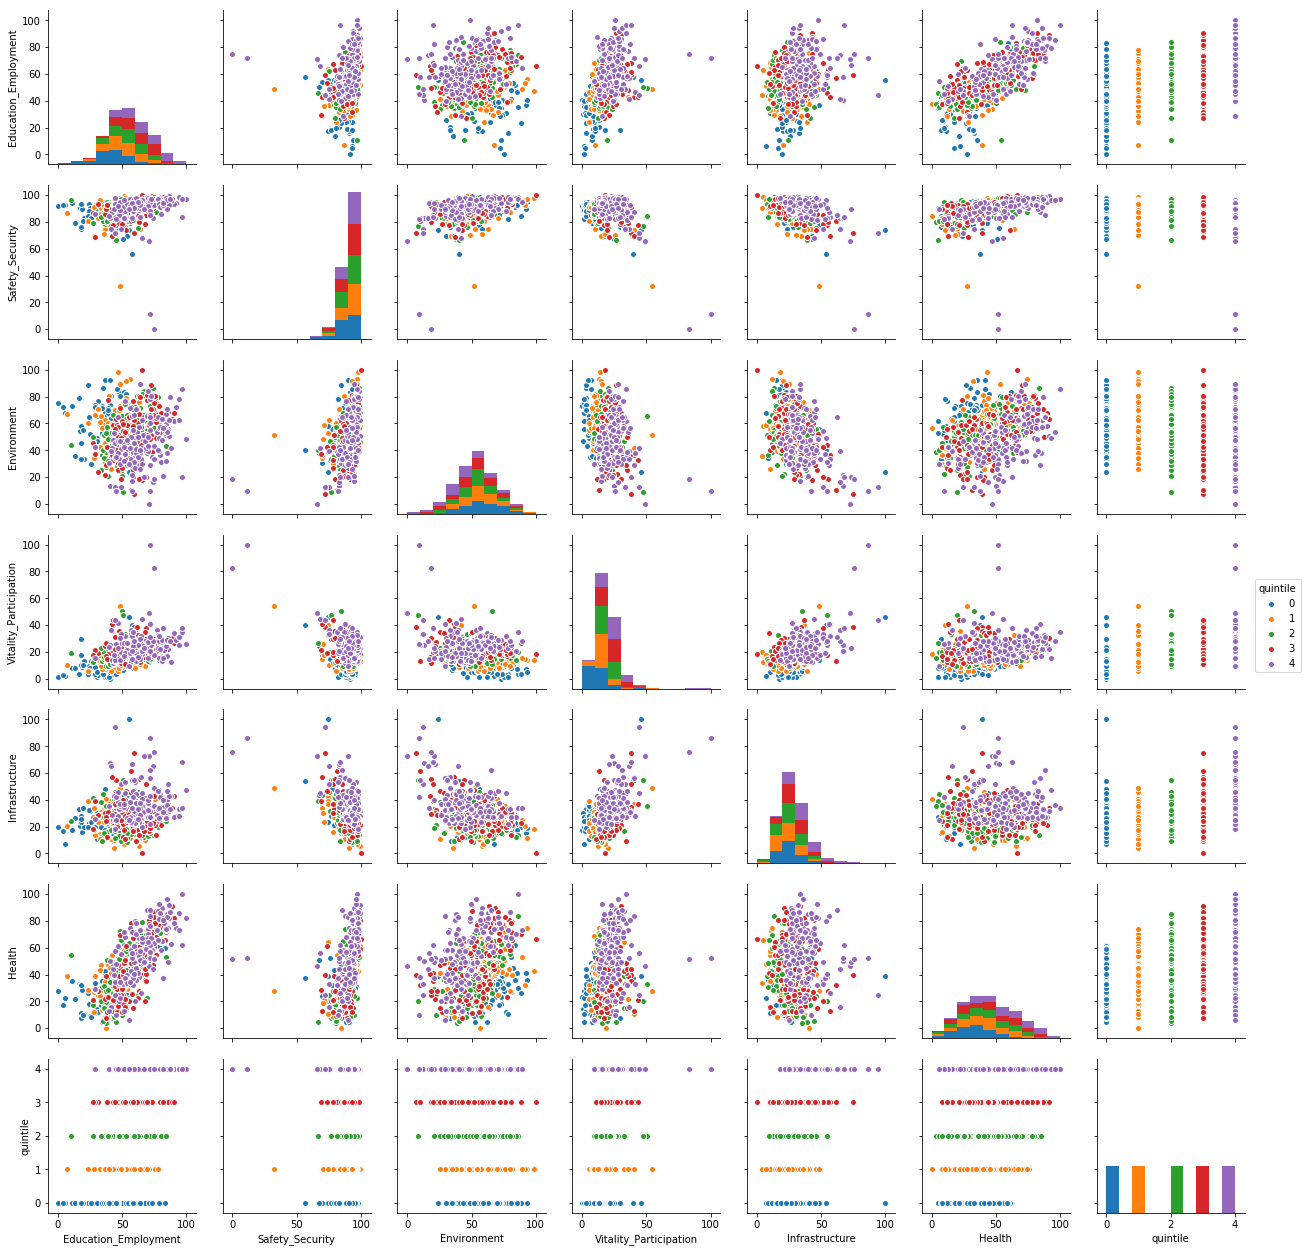
\includegraphics[scale=0.3]{figures/pairplot_quintile} % Pair-wise plot with median prices by quintile

By using the pair-wise plot and colouring the points by quintile, it is clear that there is no clear separation of quintile for any of the indicators with a more gradual movement from first to fifth quintile for most domains. Environment and Saftey and Security have an almost inverse relationship with the quintiles. Because the majority of the high-priced wards are centrally located, this may relate to a lack of greenspace and higher polution centrally as well as providing high-value targets for crime. 

? FINISH WRITING UP CLASSIFICATION MODELLING ?


%----------------------------------------------------------------------------------------
%	SECTION 5
%----------------------------------------------------------------------------------------

\section{Encoding as geoJSON}

To use the information from the creation of the well-being domains and the predictions obtained from the models in a javascript based visualisation, the information needed to be converted from a pandas dataframe in Python to a geoJSON file in javascript. A geoJSON file is a variation on the JSON format as defined below:

? GEOJSON DEFINITION ?

Whilst a relatively straightforward task within the geopandas module in Python, geoJSON accepts coordinates in latitude and longditude and the shapefile being used has the coordinates defining the ward polygons in Ordnance Survey grid references. To change this to latitude and longditude required the creation of a function that would take each polygon in the ward geometry in the geo data frame and break this down into the individual points which define the polygon. Once separated into coordinate pairs, these pairs could be reprojected to be latitude and longditude. The function was then required to recombine all of the coordinate pairs into the correct polygon geometries.

? CODE SNIPPET?

The information was then in the required format to be exported to a geoJSON file.

%----------------------------------------------------------------------------------------
%	SECTION 6
%----------------------------------------------------------------------------------------

\section{Interactive maps}

For the production of the interactive map which serves as the user front end for this project, the information was moved from the Python environment via geoJSON and into javascript functions embedded into html. This decision was made on the basis of the additional functionality and interactivity that could be smoothly added to the map in javascript. With less experience of javascript as a programming language, the leaflet.js tutorial ?INSERT REFERENCE? was an excellent starting point.

? SCREENSHOT OF MAP (not used in trailer) - MAYBE ZOOMED IN?

The map has key functionality added. This includes a zoom facility and hovering over any of the 625 wards will display the median house price value and quintile, the scores for each of the six well-being domains and the predictions from both the regression and classification models.







 

%----------------------------------------------------------------------------------------
%	THESIS CONTENT - APPENDICES
%----------------------------------------------------------------------------------------

\appendix % Cue to tell LaTeX that the following "chapters" are Appendices

% Include the appendices of the thesis as separate files from the Appendices folder
% Uncomment the lines as you write the Appendices

\include{Appendices/AppendixA}
%\include{Appendices/AppendixB}
%\include{Appendices/AppendixC}

%----------------------------------------------------------------------------------------
%	BIBLIOGRAPHY
%----------------------------------------------------------------------------------------

\printbibliography[heading=bibintoc]

%----------------------------------------------------------------------------------------

\end{document}  